% =========================================================================
% Paper 20 (A3): Distilling a frozen TSFM teacher into lightweight students
% Title direction locked at 5.3 (2026-10-04); final wording after confirm set.
% Journal target: The Journal of Supercomputing (Springer) — sn-jnl class.
% =========================================================================
\documentclass[pdflatex,sn-basic,Numbered]{sn-jnl}

\usepackage{graphicx}
\usepackage{multirow}
\usepackage{amsmath,amssymb}
\usepackage{xcolor}
\usepackage{manyfoot}
\usepackage{booktabs}
\usepackage{threeparttable}
\usepackage{float}

\begin{document}

\title{Distilling Frozen Time-Series Foundation Model Teachers into
Lightweight Edge Anomaly Detectors: A Preregistered Quality--Fidelity--Cost
Study}

\author*[1]{\fnm{Yao} \sur{Zhang}}\email{zhangyao@bdu.edu.cn}
\author[1]{\fnm{Yanling} \sur{Li}}
\author[2]{\fnm{Yichen} \sur{Wang}}
\affil[1]{\orgname{Department of Artificial Intelligence, Baoding University}, Baoding, China}
\affil[2]{\orgname{Department of Education, Baoding University}, Baoding, China}

\abstract{When a frozen time-series foundation model is distilled into a
lightweight edge student, the bottleneck sits at the distillation
interface, not at distillation itself.
This preregistered study covers 29 preregistered flows plus one
extension source, eleven arms, and 1{,}856 runs.
Students trained on the teacher's scores transfer almost none of its
ranking behavior (median Spearman $\rho = 0.184$).
All confirmatory comparisons are non-significant at the nine held-out
sources.
Switching to the teacher's forecasts as the target recovers most of the
gap on development flows.
Three teacher families agree that ranking fidelity spans near zero to
0.99 while no family gains detectable quality.
Students run 200--1500$\times$ faster per point than the teacher on
trained artifacts, and quantized PatchMLP students fit sub-millisecond,
sub-megabyte budgets.
On a Raspberry~Pi~4B students measure 0.44 to 15.47\,ms p95 while the
teacher needs 2.4\,s per point.
Zero-tuning classical scorers top the held-out macro.}\keywords{time series anomaly detection \sep knowledge distillation \sep time-series
foundation models \sep edge deployment \sep ONNX quantization \sep preregistered evaluation}

\maketitle

% ---------------------------------------------------------------
\section{Introduction}\label{sec:intro}

Time-series anomaly detection (TSAD) at the edge faces a persistent
trade-off. Detection quality demands expressive models. Latency,
memory, and storage budgets cap what can be deployed. Time-series
foundation models (TSFMs) such as Chronos, TimesFM, and Moirai add a
new option. Used zero-shot through a forecasting-residual pipeline, a
frozen TSFM scores anomalies on unseen streams with no per-device
training. Here ``edge'' denotes sub-millisecond, sub-megabyte inference
on exported artifacts. On-device validation on a Raspberry~Pi~4B
replicates the desktop protocol at the reference dimension
(Sections~\ref{sec:confirm-cost} and~\ref{sec:limitations}).

Figure~\ref{fig:boundary} sketches the deployment question.
Three candidate interfaces move the frozen teacher's signal into a
compact student during offline training, and only the student artifact
reaches the edge device.
Zero-shot audits paint a conditional picture. Frozen TSFMs are
competitive on some sources, weak on others, and orders of magnitude
more expensive to run than classical detectors.

This paper examines the natural next step. If the teacher is strong
but heavy, distill it into a lightweight student and deploy the student
at the edge. The proposal sounds straightforward, and its components
exist. Knowledge distillation for anomaly detection is established,
though the teacher there is domain-adapted and remains in the inference
loop. TSFM compression is established on the forecasting side. What is
missing is a disciplined answer to the deployment question itself. When
the teacher's detection behavior is moved into a compact student
($\approx$0.27M parameters at the reference dimension, scaling with
channel count) that must run without the teacher, does anything of value
transfer? Is the result competitive with strong classical baselines
under the same resource budget?

We answer this question with a preregistered study. We lock a causal
scoring structure on a frozen Chronos-Bolt teacher, with model-specific
point-forecast extraction when other teacher families are compared. We define three
evaluation axes: quality measured by the volume under the
precision--recall surface (VUS-PR), fidelity to the teacher's scoring
behavior, and edge cost on exported artifacts. We train eleven arms on
20 development flows from source-blocked collections. These include
score-level and ranking-level distillation of the teacher's scores, a
forecast-distillation control, self-supervised students that never see
the teacher, a linear floor, a fixed-configuration PCA baseline, and
the teacher itself. We then confirm the preregistered arms at 10
seeds on 9 held-out sources. In total: 1{,}270 preregistered training
runs across 29 flows from 22 data collections, with the full
preregistration and its revision log in the artifact package.

\begin{figure}[t]
\centering
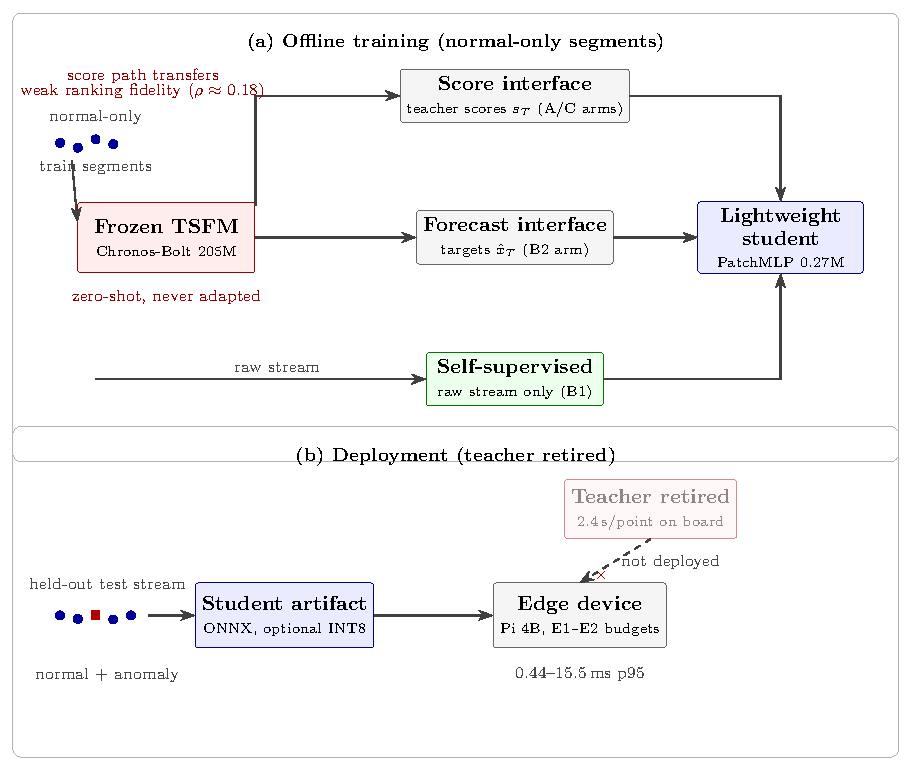
\includegraphics[width=\textwidth]{figures/fig_boundary.pdf}
\caption{Mechanism overview. (a)~Offline training: a frozen TSFM teacher
feeds three candidate interfaces (its anomaly scores, its point forecasts,
or no teacher signal at all) into a compact student trained on normal-only
segments. (b)~Deployment: only the exported student artifact runs on the
edge device; the teacher is retired and never deployed. The score
interface transfers little ranking fidelity.}
\label{fig:boundary}
\end{figure}

The answer, under this protocol, is a
\emph{delineated boundary} rather than a blanket verdict, and its
location is instructive.
The distillation \emph{interface} decides what transfers.
Score-level distillation transfers little
of the teacher's ranking behavior (median $\rho = 0.184$) and shows no
statistically detectable quality advantage; the study is powered to
rule out only large differences. On held-out sources the score arm is
the weakest of the six student arms, behind self-supervised students
and behind a linear predictor. Replacing the
score target by the teacher's \emph{forecast} closes most of the
deficit on the development set and is equivalent to
self-supervision on held-out sources. Four controls (shuffled-teacher,
equal-context, anomaly-exposure, and a second teacher family) trace
the failure to the score interface itself. The teacher is simultaneously
200--1500$\times$ slower per
point than its students and no better than the strongest of them on
held-out sources. The fixed-configuration PCA baseline tops the macro
table on certain anomaly morphologies but fails catastrophically on
others that the students handle.
Three zero-tuning classical scorers added under the final revision
 sharpen the classical anchor: two of them top the held-out macro
above every neural arm, while trained students keep a clear advantage
on the highest-channel source. What remains valuable is conditional:
score-distilled students occupy a niche on persistence-type anomalies
where both the teacher's signal and temporal structure matter.

Our contributions are fourfold. (C1)~A preregistered, source-blocked
evaluation protocol for TSFM-teacher distillation into edge students,
covering quality, fidelity, and deployment cost on exported ONNX
artifacts with optional INT8 quantization and explicit E1/E2 edge
budget tiers. (C2)~A mechanism-level boundary delineation. The
distillation interface, not distillation itself, decides what
transfers. Score-level distillation transfers little fidelity and no
detectable quality advantage over self-supervision. (C3)~The interface
analysis itself. The teacher's \emph{forecast} target is equivalent to
self-supervision while its \emph{score} target is not, with
shuffled-teacher, equal-context, anomaly-exposure, and second-teacher
controls attributing the failure to the score interface. (C4)~A
practitioner selection table mapping anomaly morphologies and resource
budgets to detectors. All artifacts are released with the
submission at \url{https://github.com/moonzymoon/tsfm-distillation-artifacts}
and archived with the Zenodo DOI 10.5281/zenodo.23623799.

% ---------------------------------------------------------------
% ---------------------------------------------------------------------------
% Section 2: Related Work (five lines, cutting sentences locked 2026-10-03)
% ---------------------------------------------------------------------------
\section{Related Work}\label{sec:related}

\subsection{Knowledge Distillation for Anomaly Detection}
Knowledge distillation (KD)~\cite{hinton2015kd} entered anomaly detection as a
\emph{detection mechanism}: a pre-trained teacher and a student of identical
capacity are both trained on normal data, and test-time anomalies are flagged
by the divergence between their outputs. This teacher--student paradigm is
established in the image domain~\cite{unifiededge2024} and, for time
series, AnomalyLLM~\cite{anomalyllm2024} adapts a large-language-model teacher
to the target domain and scores anomalies by teacher--student divergence,
claiming the first KD-based time-series anomaly detector. Multi-teacher KD for anomaly detection~\cite{ma2023multiteacher} extends the
paradigm in the Journal of Systems Architecture, and attention-based TSAD
frameworks such as IA-AD appear in The Journal of Supercomputing~\cite{iaad2025}. These detectors are single-model systems trained per domain, not distilled edge
students with a teacher-exit deployment path. Our setting differs
on all three defining axes. First, the teacher is a \emph{frozen}
time-series foundation model (TSFM) used \emph{zero-shot}: it is never adapted
to the target domain, and its anomaly scoring pipeline is fixed in advance.
Second, distillation serves as \emph{model compression} rather than as the
scoring mechanism. The student replaces the teacher entirely at inference
time, whereas mechanism-style KD keeps the teacher in the inference loop.
Third, we evaluate the resulting trade-off along quality, fidelity, and cost
axes under explicit resource budgets, which mechanism-style studies do not
consider.

\subsection{Compressing and Distilling Time-Series Foundation Models}
On the forecasting side, compressing TSFMs is well explored:
the Chronos family introduces Chronos-Bolt, an efficient
encoder-only variant~\cite{ansari2024chronos}. DistilTS~\cite{distilts2026} distills TSFM forecasting
capability (output and hidden alignment under difficulty-aware sample
weighting) into compact students. TTM~\cite{ekambaram2023ttm},
SparseTSF~\cite{hui2024sparsetsf}, and FITS~\cite{xu2024fits} build tiny
forecasters from scratch. TinyCast~\cite{tinycast2026} reaches 146K-parameter
zero-shot probabilistic forecasting with computed periodicity and
depthwise-separable convolutions, without distillation.
Concurrent work explores the opposite direction, keeping the TSFM in
the inference loop: ChronosAD~\cite{chronosad2026} uses Chronos as a
zero-shot feature extractor with a temporal refinement head, at the
cost of a foundation model at inference time. On the
classification side, TinyCN~\cite{tinycn2026} distills the Mantis
foundation model~\cite{mantis2025} into tiny convolutional classifiers. None
of these works distills \emph{detection} behavior, and a forecaster distilled
for point accuracy need not preserve anomaly-scoring behavior; we therefore
treat ``forecast-distillation-then-residual'' as an explicit control arm
(B2) rather than assuming it equivalent to score distillation. Concurrent
domain-specific work distills fine-tuned industrial foundation models for
particle-physics trigger hardware~\cite{ancone2026daq}; it neither addresses
general-purpose anomaly detection nor uses frozen zero-shot teachers.

\subsection{TSFMs as Zero-Shot Anomaly Detectors}
Systematic evaluations show that frozen TSFMs can act as zero-shot anomaly
detectors through forecasting-residual pipelines, but with strongly
condition-dependent reliability. Aggregated evaluations over public
benchmarks~\cite{tsfmad2024eval} and the TSB-AD suite~\cite{tsbad2024} report
large variance across datasets, and continuous (level-shift) anomalies are a
known failure signature~\cite{uray2026}. A leakage-aware evaluation protocol
with a lightweight trainable head over frozen TSFM
representations~\cite{clra2026} reaches conclusions consistent with
representation--detectability gaps. These studies characterize \emph{how good
the teacher is}; none asks whether that behavior can be moved into a
deployable student. Our protocol reuses their interface design (Section
\ref{sec:protocol}) and cites their numbers as teacher priors, while the
fidelity--quality analysis is complementary to their audit perspective.

\subsection{Lightweight Time-Series Anomaly Detection}
Lightweight TSAD spans classical baselines (Matrix
Profile~\cite{matrixprofile2016}, PCA reconstruction, LOF, one-class SVM),
compact neural detectors, and edge-oriented systems that combine KD with
quantization~\cite{unifiededge2024}. Benchmark suites score such methods on
accuracy, with TSB-AD~\cite{tsbad2024} and TAB~\cite{tab2025} using
VUS-PR~\cite{vus2022} as the primary metric, but do not couple accuracy to
latency, model size, or memory budgets, and edge-oriented TSAD papers
typically report custom efficiency metrics. The combination of a fixed
accuracy benchmark with explicit resource-constraint tiers and a preregister
protocol is, to our knowledge, open territory; our three-axis evaluation
framework is designed to occupy it.

\subsection{Positioning}
In summary, existing work provides (i) the KD-AD lineage whose teachers are
domain-adapted and remain in the inference loop, (ii) TSFM compression for
forecasting and classification, (iii) audits of frozen TSFMs as detectors,
and (iv) accuracy-only lightweight benchmarks. What is missing is a
preregistered answer to the deployment question. When a frozen TSFM's
detection behavior is distilled into a compact student that
must run without the teacher, what actually transfers, and is the result
competitive with strong classical baselines under the same resource budget?
Section~\ref{sec:protocol} defines our protocol for answering this, and
Sections~\ref{sec:dev-results} and~\ref{sec:confirm} report the answer, including a
prominent boundary delineation. The score interface fails to transfer, the forecast interface does not.

% ---------------------------------------------------------------------------
% Section 3: Preregistered Protocol (slimmed: implementation/data details
% moved to Section 4 Experimental Setup per venue convention)
% ---------------------------------------------------------------------------
\section{Preregistered Protocol}\label{sec:protocol}

The protocol was preregistered (v1.0, with an append-only revision log
R1--R5 disclosed in Section~\ref{sec:limitations-revision} and the full
hash chain in Appendix~\ref{app:hashchain}) \emph{before} any
test-segment metric was computed; the confirmation-set arm list was
amended in R5 based on dev-set evidence only, with the ruling preceding
the launch of the confirmation runs and the confirmation data untouched
throughout. This section states the locked decisions; datasets,
implementation details, and the statistical protocol are specified in
Section~\ref{sec:setup}.

\subsection{Detection Interface (Teacher Lock)}\label{sec:interface}
The teacher is a frozen TSFM combined with a fixed, causal detection
pipeline: (i)~context-wise $z$-normalization using statistics of the
context window only; (ii)~one-step probabilistic forecasting of $x_t$
from $x_{<t}$, with the \emph{median} quantile taken as the point
forecast (uniform across model families); (iii)~per-channel absolute
residuals $|x_{t,c}-\hat{x}_{c}(t)|$; (iv)~cross-channel aggregation by
\emph{max}. The teacher score is therefore $s_T(t)=g(x_{\le t})$;
quantile-interval scoring is deliberately excluded (interface
sensitivity belongs to our companion audit). Context length is each
model's library default and is recorded in the cache metadata.
Distillation aligns the student to exactly this interface. The student
input window ends at the same timestamp the teacher scores, so student
and teacher scores are timestamp-aligned by construction. After
training, the teacher is removed from the deployment path entirely, and the
student is the only inference-time artifact. Input windows are
leakage-audited by arm: score-distilled students (A/C) receive the
window $x_{t-L+1..t}$ \emph{including} the current observation $x_t$,
whereas the regression arms (B1/B2) receive $x_{t-L..t-1}$ and predict
$x_t$, so the prediction target never enters the input. The teacher
scores with a 512-point context and the students with 128-point
windows; the interface ablation at $L{=}512$ (R7, exploratory, five flows)
does not support this asymmetry as the driver of the ladder conclusion
(four of five flows), though full information-set
equalization across all arms remains future work. Figure~\ref{fig:pipeline} summarizes the locked design.

\begin{figure}[t]
\centering
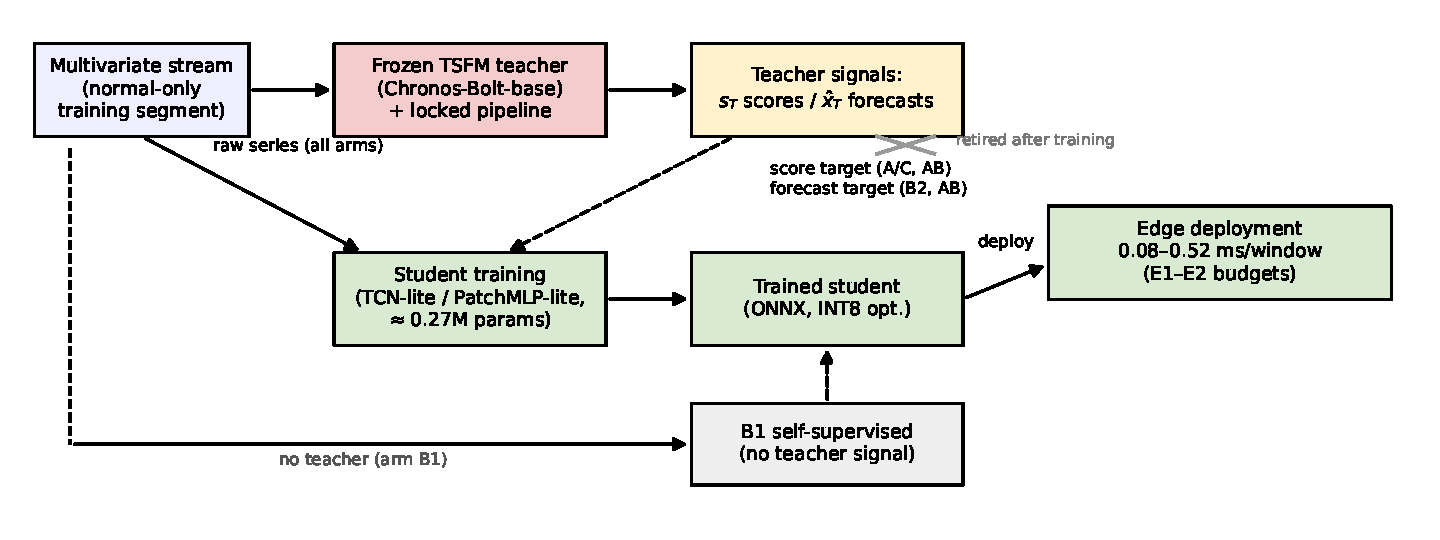
\includegraphics[width=\textwidth]{figures/fig_pipeline.pdf}
\caption{Study design. The frozen TSFM teacher (Chronos-Bolt-base behind the
locked causal scoring interface of Section~\ref{sec:interface}) provides two
candidate distillation signals to the student training stage: its anomaly
scores $s_T$ (arms A/C and the AB hybrid) and its point forecasts
$\hat{x}_T$ (arm B2 and AB). Arm B1 receives no teacher signal and trains
on the raw stream only. After training,
the teacher is retired. Only the exported student artifact (ONNX, optional
INT8) is deployed and timed.}
\label{fig:pipeline}
\end{figure}

\subsection{Three-Axis Evaluation Framework}\label{sec:axes}
All arms are evaluated on three axes. \textbf{Quality} is VUS-PR
(primary) and VUS-ROC (secondary), never using point adjustment or
thresholded $F_1$. \textbf{Fidelity} measures how faithfully the student
reproduces the teacher's scoring behavior (full-series and tail-restricted
rank agreement); it is a diagnostic axis, reported even when it conflicts
with quality. \textbf{Cost} is measured on exported inference artifacts
(ONNX, optional INT8), never on training checkpoints, under a
single-thread deployment protocol with full environment disclosure.
Formal definitions, tools, and protocols are tabulated in
Table~\ref{tab:metrics}.

\subsection{Arms and Controls}\label{sec:arms}
The preregistered arms are: the \textbf{score arm (A)}, regressing a
Huber loss to the teacher score $s_T$; the \textbf{ranking arm (C)}, a
RankNet-style objective~\cite{burges2005ranknet} over sampled within-stream pairs (relational distillation in the spirit of RKD\cite{park2019rkd}); the
\textbf{self-supervised control (B1)}, training the same backbone by
next-step regression \emph{without any teacher signal}; the
\textbf{forecast-distillation control (B2)}, regressing the teacher's
point forecast (DistilTS-style); the \textbf{hybrid (AB)}, coupling the
score objective with a $\lambda$-weighted forecast-alignment term; a
\textbf{linear floor}; and fixed references, namely the frozen teacher (T0)
and a fixed-configuration PCA-reconstruction baseline fitted on the
training segment only. Causal Matrix Profile and LOF were designated as auxiliary classical
baselines. Causal Matrix Profile was ultimately not executed (deviation
disclosed in R5): a faithful causal implementation with the full tuning
budget was judged disproportionate to its marginal value. LOF was later
added in a window-feature form under revision R11, fit on the full
unlabeled test segment (transductive, non-streaming), alongside two
zero-tuning streaming scorers. Full arm definitions, the
comparison table, and implementation details are in
Section~\ref{sec:setup-arms}.

\subsection{Preregistration and Staging}\label{sec:staging}\label{sec:limitations-revision}
The study proceeds in two source-blocked stages: an \emph{exploration} stage
on 20 development flows (arm selection, ablations, mechanism controls)
and a \emph{confirmation} stage on 9 held-out flows from source-blocked
collections (one disclosed NAB exception), at increased seed count
(3 seeds per arm on development auxiliary arms, 10 on the confirmation
stage). The preregistration was amended five
times through the append-only log (R1--R5), each before the affected
measurements and each disclosed with its trigger in the revision
history; three further revisions (R6--R8) registered exploratory
controls after the confirmation stage began, and are flagged as such in
the hash chain (Appendix~\ref{app:hashchain}). The confirmatory analyses are exactly the three preregistered
pairwise comparisons of the confirmation stage, and all other analyses
(macro rankings, conditional morphology analysis, the selection table,
and the shuffled-teacher control) are exploratory and labelled as such.
Sibling-project reuse of teacher caches is disclosed, as is the fact
that the teacher pipeline configuration is shared with a companion
audit study.


% ---------------------------------------------------------------------------
% Section 4: Experimental Setup (split from preregistered protocol per JoS
% convention: setup chapter separate from protocol chapter)
% ---------------------------------------------------------------------------
\section{Experimental Setup}\label{sec:setup}

\subsection{Data: Flows and Source Blocking}\label{sec:setup-data}
The evaluation grid (Table~\ref{tab:flows}) covers 29 preregistered flows drawn from 22 original
data collections, split into 20 development flows (exploration and arm
selection) and 9 confirmation flows whose sources are source-blocked from the
development set. Labels are the official protocol labels of each
collection throughout; flows whose test segments contain no anomalies are
excluded from VUS computation and reported as such. Multivariate flows
are reduced to per-window scores by the teacher aggregation
(Section~\ref{sec:interface}); univariate flows are scored directly.
Every flow trains on its unlabeled training segment and is evaluated on
its disjoint test segment; source-block splits keep the two stages
disjoint with one disclosed exception (the NAB collection contributes
streams to both stages). One further caveat is disclosed: SWaT and WADI
share an operator testbed lineage, and the NAB
collection contributes several streams to the development set while one
NAB-derived stream appears in confirmation.

\begin{table}[t]
\centering
\caption{Evaluation metrics and protocols per axis. VUS-ROC and the
tail-agreement companions are computed and shipped with the per-run
artifacts; the paper text reports VUS-PR, $\rho$, and top-5\% overlap.}
\label{tab:metrics}
\scriptsize
\begin{tabular}{p{1.7cm}p{3.1cm}p{2.3cm}p{2.6cm}}
\toprule
Axis & Metric & Tool / protocol & Notes \\
\midrule
Quality & VUS-PR (primary), VUS-ROC (secondary; artifact-only) & official VUS implementation, default buffering & no point adjustment; no thresholded $F_1$ \\
Fidelity & Spearman $\rho$; top-1\%/5\% overlap; pairwise agreement; tail rank agreement (artifact-only) & per-window scores vs.\ teacher scores & reported even when conflicting with quality \\
Cost & p50/p95 latency per window; file size; peak RSS & single-thread ORT, batch 1; matrix re-timed on trained artifacts, 5 rounds $\times$ (50 warm-up + 500 timed), Appendix~\ref{app:cost} & cold-start excluded (disclosed) \\
Equivalence & TOST-style interval reading & preregistered margin 0.05 VUS-PR & bootstrap CIs, 5{,}000 resamples \\
\bottomrule
\end{tabular}
\end{table}\begin{table}[t]
\centering
\caption{Evaluation flows. Dev$=$development (exploration and arm
selection); Conf$=$confirmation (held-out sources). Channels are the
per-window input dimensionality; test points and AR (point-label anomaly
ratio) refer to the evaluated test segment.}
\label{tab:flows}
\setlength{\tabcolsep}{3pt}
\scriptsize
\setlength{\tabcolsep}{2.2pt}
\begin{tabular}{p{1.3cm}p{2.55cm}rrrp{0.9cm}}
\toprule
Stage & Flow & Collection & Channels & Test points & AR \\
\midrule
Dev & SWaT (SWaT-id1) & SWaT testbed & 66 & 5{,}474 & 0.363 \\
Dev & HAI 2.2 & HAI & 86 & 86{,}400 & 0.010 \\
Dev & SMD machine-4 & Server Machine Dataset & 38 & 18{,}096 & 0.024 \\
Dev & SMD machine-20 & Server Machine Dataset & 38 & 6{,}123 & 0.026 \\
Dev & PSM & Pooled Server Metrics & 25 & 87{,}752 & 0.278 \\
Dev & MSL-10 / MSL-5 & NASA MSL & 55 & 1{,}510 / 3{,}804 & 0.087 / 0.111 \\
Dev & SMAP-4 / SMAP-13 & NASA SMAP & 25 & 2{,}191 / 1{,}943 & 0.055 / 0.026 \\
Dev & GHL-2 & Gas Heating Loop & 19 & 149{,}000 & 0.012 \\
Dev & SVDB-2 & MIT-BIH SVDB (ECG) & 2 & 175{,}418 & 0.049 \\
Dev & EMG & EMG (Lobov et al.) & 8 & 130{,}900 & 0.057 \\
Dev & J-D service-0 & JumpStarter KPI & 38 & 23{,}705 & 0.004 \\
Dev & NAB cpu-24ae8d / cpu-53ea38 & NAB AWS & 1 & 2{,}016 each & 0.115 / 0.319 \\
Dev & NAB occupancy-6005 & NAB realTraffic & 1 & 1{,}190 & 0.001 \\
Dev & NAB machine\-temp & NAB realKnownCause & 1 & 11{,}348 & 0.280 \\
Dev & Exathlon-1 & Exathlon & 18 & 30{,}476 & 0.178 \\
Dev & Opportunity & OPP wearable & 248 & 1{,}375 & 0.240 \\
Dev & GECCO & GECCO water quality & 9 & 55{,}409 & 0.004 \\
\midrule
Conf & WADI (A1 train / A2 attack) & WADI & 116 & 172{,}803 & 0.058 \\
Conf & Genesis & JSA Vol.\,143 slice & 18 & 682 & 0.073 \\
Conf & Daphnet & Daphnet wearable & 9 & 18{,}042 & 0.128 \\
Conf & MGAB & MGAB synthetic & 1 & 50{,}000 & 0.003 \\
Conf & Yahoo-A3 & Yahoo A3 benchmark & 1 & 840 & 0.007 \\
Conf & IOPS & IOPS KPI & 1 & 74{,}565 & 0.005 \\
Conf & MITDB-5 & MIT-BIH Arrhythmia (ECG) & 2 & 63{,}087 & 0.007 \\
Conf & NEweather & NEweather & 8 & 9{,}079 & 0.326 \\
Conf & NAB exchange-2-cpm & NAB realAdExchange & 1 & 812 & 0.201 \\
\bottomrule
\end{tabular}
\end{table}

\subsection{Arms and Reference Baselines}\label{sec:setup-arms}
Table~\ref{tab:arms} summarizes the compared arms, their training
signals, and their inference-time footprint. All neural arms share the
two compact ($\approx$0.27M-parameter) backbones; the linear floor and PCA serve as
non-neural references. The frozen teacher (T0) is a reference only and
never participates in deployment.

\begin{table}[t]
\centering
\caption{Compared arms. ``Teacher at inference'' indicates whether the
frozen TSFM must be present when the arm produces anomaly scores on the
test segment; only the deployed students and the classical references
run without it.}
\label{tab:arms}
\scriptsize
\begin{tabular}{p{2.2cm}p{3.1cm}p{2.0cm}p{1.5cm}p{1.7cm}}
\toprule
Arm & Training signal & Backbone & Teacher at train & Teacher at inference \\
\midrule
T0 (teacher) & --- (zero-shot) & Chronos-Bolt-base & --- & \textbf{yes} \\
A (score) & teacher scores $s_T$ & TCN / PatchMLP & yes & no \\
C (ranking) & teacher score ranking & TCN / PatchMLP & yes & no \\
B1 (self-sup.) & next-step residuals & TCN / PatchMLP & no & no \\
B2 (forecast dist.) & teacher point forecasts & TCN / PatchMLP & yes & no \\
AB (hybrid) & scores + $\lambda$ forecast align. & TCN / PatchMLP & yes & no \\
LINEAR (floor) & next-step residuals & linear & no & no \\
PCA (fixed config.) & train-segment fit (95\% var.) & --- & no & no \\
\bottomrule
\end{tabular}
\end{table}

\subsection{Implementation and Training Details}\label{sec:setup-impl}
Table~\ref{tab:hyper} lists the training configuration; per-flow manifests
with the exact values are part of the artifact package. Students are
trained on a single RTX 5060 Ti (16\,GB); edge timing uses single-thread
ONNX Runtime 1.28 on the desktop CPU (12th-Gen Intel Core i7-12700F),
with PyTorch 2.13 for training; the teacher scores on the same GPU.

\begin{table}[t]
\centering
\caption{Training and export configuration (identical across arms unless
stated).}
\label{tab:hyper}
\scriptsize
\begin{tabular}{p{3.4cm}p{8.5cm}}
\toprule
Item & Value \\
\midrule
Window length $L$ & 128 (standard); 512 (interface ablation, R7) \\
Stride & 2 (training window sampling) \\
Optimizer & Adam, lr $10^{-3}$ \\
Batch size & 256 (A/C scoring arms); 256 (B1/B2); 128 (L=512 ablation) \\
Epochs & 30, per flow, per seed \\
Seeds & 5 (main grid); 3 (auxiliary arms); 10 (confirmation) \\
Backbone parameters (66-ch) & TCN-lite 272{,}401; PatchMLP-lite 265{,}617; linear 8{,}383 \\
Teacher & Chronos-Bolt-base, context 512, median-quantile point forecast; \\
 & TimesFM 2.5-200M, context 1024, mean point output (secondary subset) \\
Export & ONNX opset 17, dynamic batch, optional dynamic INT8 \\
Edge timing & single-thread ORT, batch 1, p50/p95 over 200 windows \\
\bottomrule
\end{tabular}
\end{table}

\subsection{Evaluation Metrics and Statistical Protocol}\label{sec:setup-metrics}
Table~\ref{tab:metrics} defines the three axes. Statistics operate at the
source level. Per-flow seed-averaged scores are compared with two-sided
exact Wilcoxon signed-rank tests under Holm correction across the
three preregistered comparisons (raw and adjusted $p$ both reported in
Section~\ref{sec:confirm-comparisons}, together with the exact test's
minimum attainable $p$ at $n{=}9$), effect sizes via
matched-pairs rank-biserial correlation (on ranks of absolute paired
differences, with sign counts alongside) and raw differences with
source-level bootstrap 95\% CIs, and vote counts. Equivalence claims use
the preregistered 0.05 VUS-PR margin (TOST-style interval reading on
the 95\% CI, which is more conservative than the standard 90\% TOST
band). Exploratory analyses that resample at the flow level (e.g., the
shuffled-teacher control) are annotated as such and do not feed the
source-level claims.
Any claim of ``retaining teacher performance'' requires this margin with
interval support. Negative results are reported in full. For clarity,
the \emph{confirmatory} analyses are exactly the three preregistered
pairwise comparisons of the confirmation stage; macro rankings, the
conditional morphology-level analysis, and the practitioner selection
table are \emph{exploratory} and labelled as such wherever they appear.






\begin{figure}[t]
\centering
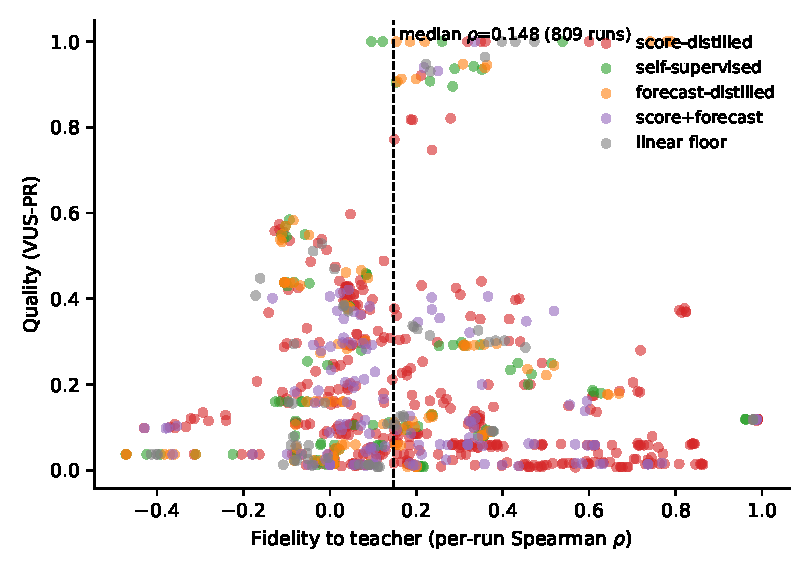
\includegraphics[width=0.8\textwidth]{figures/fig_fidelity_quality.pdf}
\caption{Fidelity--quality decoupling. Each point is one training run
with finite fidelity (809 runs: 389 main-grid plus 420 auxiliary-arm
runs; per-run Spearman $\rho$ against the teacher vs.\ that run's
VUS-PR), colored by
distillation-signal family. The dashed line is the median over all
plotted runs ($\rho = 0.148$); the median over the 389 main-grid runs
alone is 0.184 (Section~\ref{sec:dev-fidelity}). High quality does not require high fidelity; where fidelity is
high, students inherit the teacher's level, including its weaknesses.}
\label{fig:fidelity}
\end{figure}

% ---------------------------------------------------------------------------
\section{Results on Development Flows}\label{sec:dev-results}
\noindent
{\bfseries RQ1 (quality).} Does the teacher improve detection quality over students trained without it, and does the answer depend on which teacher signal is distilled? {\bfseries RQ2 (fidelity).} Does score distillation transfer the teacher's scoring behavior? {\bfseries RQ3 (attribution).} Is any failure attributable to the score interface itself, rather than to context asymmetry, teacher capacity, or the training constraint?
% ---------------------------------------------------------------------------

This section reports the exploration stage on the 20 development flows:
the preregistered main grid (arms A/C $\times$ two backbones $\times$ 5
seeds), the auxiliary arms at 3 seeds (B1, B2, AB, LINEAR), and the fixed
references (frozen teacher T0, PCA). All 820 training runs completed without
failure; per-flow seed dispersion is included in the artifact package.

\subsection{The Full Picture}\label{sec:dev-picture}
Table~\ref{tab:dev} reports VUS-PR for eleven arms, the teacher, and PCA
across all development flows. Three observations structure everything that
follows. First, \emph{no method dominates}: the best per-flow arm changes
across flows, and the fixed-configuration PCA baseline (the preregistered strong
classical reference) attains the highest macro mean (0.286) and median
(0.149) while failing catastrophically on specific flow types. The gas-heating loop
is the sharpest single demonstration of the interface effect in our
data. On this one flow, the teacher, every score-distilled student
(0.008--0.013, including the AB hybrids), and PCA (0.007) all collapse,
while the two
forecast-trained students reach 0.38--0.44. Second, \emph{eight of the ten neural student arms exceed the
teacher's macro mean} (the exceptions are the two TCN variants trained
on the teacher's weakest signal, A-TCN 0.137 and AB-TCN 0.130 vs.0.165); the best per-flow student beats the teacher on 16 of 20 flows
(2 losses, 2 ties). The teacher is a weak spot on its own grid, echoing the
condition-dependence reported by zero-shot audits. Third, the \emph{interface} of the distillation signal
matters more than the presence of a teacher. Self-supervised and
forecast-distilled students (B1/B2/LINEAR, 0.217--0.253 macro) dominate
score- and ranking-distilled students (A/C, 0.137--0.180).

% AUTO-GENERATED from results/m5*/ — do not edit numbers by hand
\begin{sidewaystable}
\centering
\caption{Development-set VUS-PR (mean over seeds) for eleven arms, the frozen teacher (T0), and the preregistered PCA baseline across the 20 dev flows. Best per flow in bold.}
\label{tab:dev}
\scriptsize
\setlength{\tabcolsep}{2.4pt}
\begin{tabular}{lccccccccccccc}
\toprule
Flow & C-PM & C-TCN & A-PM & A-TCN & B1-TCN & B1-PM & B2-TCN & B2-PM & AB-PM & AB-TCN & LINEAR & T0 & PCA \\
\midrule
D10\_GHL\_id2 & 0.008 & 0.008 & 0.011 & 0.012 & 0.438 & 0.435 & \textbf{0.438} & 0.435 & 0.013 & 0.013 & 0.383 & 0.009 & 0.007 \\
D11\_SVDB\_id2 & 0.061 & 0.058 & 0.060 & 0.059 & 0.081 & \textbf{0.092} & 0.081 & 0.091 & 0.061 & 0.059 & 0.091 & 0.067 & 0.069 \\
D12\_EMG & 0.119 & 0.116 & 0.117 & \textbf{0.119} & 0.118 & 0.119 & 0.118 & 0.119 & 0.118 & 0.116 & 0.118 & \textbf{0.119} & 0.071 \\
D13\_JD1\_svc0 & 0.014 & 0.019 & 0.015 & 0.016 & 0.009 & 0.008 & 0.009 & 0.009 & 0.015 & 0.016 & 0.008 & 0.073 & \textbf{0.695} \\
D14\_NAB\_cpu24ae8d & 0.140 & 0.226 & 0.202 & 0.196 & 0.183 & 0.236 & 0.178 & 0.234 & 0.201 & 0.202 & \textbf{0.305} & 0.222 & 0.136 \\
D15\_NAB\_cpu53ea38 & 0.304 & 0.292 & 0.304 & 0.298 & 0.294 & 0.291 & 0.292 & 0.293 & 0.288 & 0.297 & 0.305 & 0.281 & \textbf{0.330} \\
D16\_NAB\_occ6005 & 0.560 & 0.108 & 0.550 & 0.018 & \textbf{1.000} & 0.483 & \textbf{1.000} & \textbf{1.000} & 0.516 & 0.017 & \textbf{1.000} & 0.200 & 0.036 \\
D17\_NAB\_machtemp & 0.297 & 0.397 & 0.350 & 0.427 & 0.457 & 0.260 & \textbf{0.459} & 0.286 & 0.344 & 0.396 & 0.334 & 0.328 & 0.284 \\
D18\_Exathlon\_id1 & 0.481 & 0.550 & 0.273 & 0.117 & 0.915 & 0.925 & 0.933 & 0.922 & 0.656 & 0.100 & 0.947 & 0.561 & \textbf{0.999} \\
D19\_OPP\_id3 & 0.202 & 0.257 & 0.180 & 0.214 & 0.160 & 0.160 & 0.160 & 0.160 & 0.176 & 0.226 & 0.158 & 0.255 & \textbf{0.439} \\
D1\_SWaT\_id1 & 0.542 & 0.524 & 0.424 & 0.396 & 0.545 & \textbf{0.568} & 0.540 & 0.567 & 0.384 & 0.350 & 0.503 & 0.331 & 0.446 \\
D20\_GECCO\_id1 & 0.015 & 0.014 & 0.011 & 0.014 & 0.014 & 0.014 & 0.014 & 0.014 & 0.013 & 0.014 & 0.013 & 0.014 & \textbf{0.403} \\
D2\_HAI & 0.013 & \textbf{0.018} & 0.014 & 0.014 & 0.016 & 0.013 & 0.015 & 0.015 & 0.014 & 0.013 & 0.012 & 0.015 & 0.013 \\
D3\_SMD\_id4 & 0.055 & 0.069 & 0.068 & 0.050 & 0.044 & 0.028 & 0.044 & 0.028 & \textbf{0.070} & 0.048 & 0.032 & 0.069 & 0.040 \\
D4\_SMD\_id20 & 0.030 & 0.061 & 0.161 & 0.099 & 0.078 & 0.023 & 0.071 & 0.023 & 0.046 & 0.084 & 0.042 & 0.030 & \textbf{0.885} \\
D5\_PSM & 0.372 & 0.416 & 0.419 & 0.392 & 0.382 & 0.381 & 0.352 & 0.383 & 0.393 & 0.350 & 0.380 & 0.388 & \textbf{0.501} \\
D6\_MSL\_id10 & 0.085 & 0.088 & 0.090 & 0.098 & 0.105 & 0.100 & 0.105 & 0.100 & 0.089 & 0.096 & \textbf{0.107} & 0.101 & 0.080 \\
D7\_MSL\_id5 & \textbf{0.207} & 0.109 & 0.155 & 0.106 & 0.129 & 0.107 & 0.126 & 0.112 & 0.151 & 0.110 & 0.126 & 0.129 & 0.162 \\
D8\_SMAP\_id4 & 0.059 & 0.060 & 0.059 & 0.059 & 0.058 & 0.060 & 0.059 & 0.060 & 0.059 & 0.060 & 0.058 & 0.065 & \textbf{0.080} \\
D9\_SMAP\_id13 & \textbf{0.037} & \textbf{0.037} & \textbf{0.037} & \textbf{0.037} & \textbf{0.037} & \textbf{0.037} & \textbf{0.037} & \textbf{0.037} & \textbf{0.037} & \textbf{0.037} & \textbf{0.037} & \textbf{0.037} & \textbf{0.037} \\
\midrule
Macro mean & 0.180 & 0.171 & 0.175 & 0.137 & 0.253 & 0.217 & 0.251 & 0.244 & 0.182 & 0.130 & 0.248 & 0.165 & 0.286 \\
Median & 0.102 & 0.098 & 0.136 & 0.099 & 0.123 & 0.113 & 0.122 & 0.115 & 0.104 & 0.090 & 0.122 & 0.110 & 0.149 \\
\bottomrule
\end{tabular}
\end{sidewaystable}

\subsection{Fidelity--Quality Decoupling}\label{sec:dev-fidelity}
If distillation transferred the teacher's scoring behavior faithfully,
the student's scores would correlate strongly with the teacher's. The data refute this. Across the 389 main-grid
runs with finite fidelity (of 400; the remainder yield constant score
vectors), the median teacher--student Spearman $\rho$ is 0.184; only 22\% of
runs exceed $\rho>0.5$, while 53\% fall below 0.2 (Figure~\ref{fig:fidelity}). The decoupling is
flow-structured rather than noise. On the three flows where the median
$\rho$ is highest (SVDB $\rho{\approx}0.84$, MSL-5 $\rho{\approx}0.70$,
J-D $\rho{\approx}0.61$), students track the teacher closely and inherit
its level of performance. On the flows where students improve most over
the teacher (e.g., SWaT: student 0.54 vs.\ teacher 0.33 with
$\rho{\approx}-0.10$; NAB-occupancy: 0.56 vs.\ 0.20; machine-temperature:
0.43 vs.\ 0.33), the student is \emph{not} imitating the teacher at all.
The mechanism is consistent with these observations, which we state as a
hypothesis rather than a proof. Under the normal-only training constraint,
the teacher's scores act as a noisy, weakly informative regression target,
and the measured gains come from the student's inductive bias filtering
this target, a regularization effect, rather than from behavioral
transfer.
The preregistered fidelity companions agree. Across the same 389 runs,
top-5\% score-set overlap averages 0.242 (median 0.151; chance
is 0.05) and pairwise agreement on non-tied teacher pairs averages
0.594, above chance but far from imitation. Anomaly-tail fidelity tells the same story from the deployment
angle and is reported per flow in the artifact package.

\subsection{The Interface Ladder}\label{sec:dev-ladder}
The preregistered three-level comparison asks \emph{which
distillation objective is strongest}. Ranking the objectives by their
information content about the anomaly (ground-truth-free self-supervision B1,
the teacher's \emph{forecast} B2, and the teacher's \emph{score} A/C)
produces a consistent macro separation
(B1/B2/LINEAR $\approx 0.22$--$0.25$ vs.\ A/C $\approx 0.14$--$0.18$),
though within the upper family the B1-vs-B2 ordering swaps with the
backbone (B2-TCN 0.251 edges out B1-PM 0.217's family range; on the
confirmation set the same comparison reverses, Section~\ref{sec:confirm-comparisons}).
Score-level distillation, the interface this paper set out to test, is the
weakest of the three; the pairwise per-flow record confirms it is not a
macro artifact (B1-TCN beats C-PM on 11 of 20 flows). Notably, a linear
predictor with residual scoring (0.248 macro) comes within 0.003 of the
strongest distilled neural student on development (B2-TCN 0.251)
and is the strongest student arm on held-out sources (0.323). The AB arm, which couples score distillation with
forecast alignment, recovers part of the gap over pure score distillation
(AB-PM 0.182 vs.\ A-PM 0.175 at macro) but remains far below
forecast-only training (B2-PM 0.244), indicating that the alignment
benefit comes from the forecast target itself rather than from the
combination.
An interface ablation (revision R7, exploratory) addresses the main
confound directly. Retraining A-PM and B1-PM at the teacher's own
context length ($L{=}512$ instead of 128) on five representative flows
leaves the ladder intact. The B1$-$A difference is $+0.148$ at
$L{=}512$ vs.\ $+0.144$ at $L{=}128$ (per-flow direction agrees on 4 of
5; the disagreement is the occupancy flow). On these five flows, the
context-length asymmetry between teacher and student does not support
an explanation of the interface gap.

A teacher-on-anomaly control (revision R8, exploratory) tests whether
the normal-only training signal, rather than the interface itself, is
the binding constraint. Synthetic anomalies (1\% spikes, 1\% 100-point
level shifts, $k\in\{3,5,8\}\sigma$) are injected into the training
segments of five representative flows; the injection parameters are chosen
independently of the students' window-residual mechanism (spike and
level-shift morphologies, not residual-shaped anomalies), so no arm is
favored by construction; the teacher scores the augmented
segments (its score discriminates injected from normal points on three
of five flows, ratios 1.2--2.8$\times$), and A-PM and B1-PM are
retrained on the augmented streams. The result is sharply bimodal
(Figure~\ref{fig:r8bimodal}).
Where the teacher discriminates, score distillation with anomaly
exposure improves dramatically (Exathlon: $0.27\to0.86$); where it does
not (occupancy: teacher ratio $<1$), augmented distillation degrades
equally dramatically ($0.55\to0.08$). The self-supervised control is
robust to the same augmentation (mean change $+0.001$, per-flow range
$-0.002$ to $+0.008$ across the five
flows). The score interface, then, is not categorically unable to
transfer detection behavior. It inherits the teacher's
condition-dependent inconsistency. Deploying it is a bet on the teacher
responding informatively to the anomalies at hand, and verifying the
bet requires running the teacher on representative data, an offline
cost that is amortized across deployments but still non-trivial
compared to fully self-supervised training.

\begin{figure}[t]
\centering
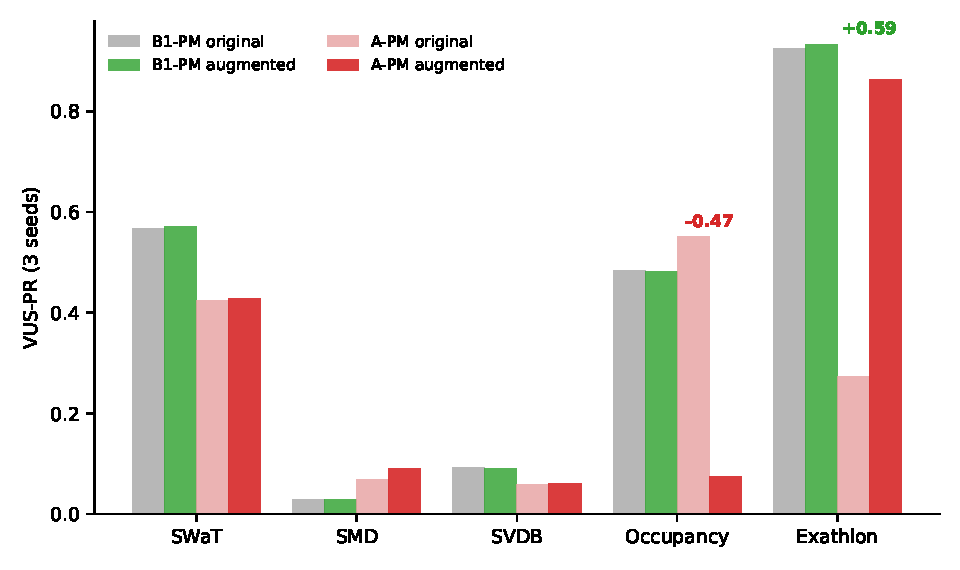
\includegraphics[width=0.8\textwidth]{figures/fig_r8_bimodal.pdf}
\caption{Teacher-on-anomaly control (R8, exploratory): VUS-PR (mean of
3 seeds) on five development flows, four bars per flow. Gray/green:
B1-PM trained on original vs.\ anomaly-augmented segments; light
red/red: A-PM original vs.\ augmented. Bold annotations give the
within-arm augmented-minus-original difference for A-PM (the same
quantity quoted in the text). The outcome is bimodal. Where the
teacher's scores discriminate the injected anomalies, augmented score
distillation improves sharply (Exathlon: $0.27\to0.86$); where they do
not (Occupancy, teacher ratio ${<}1$), it degrades sharply
($0.55\to0.08$). B1-PM is robust to the same augmentation on all five
flows.}
\label{fig:r8bimodal}
\end{figure}

\subsection{Conditional Analysis: When Is Each Arm Worth It?}\label{sec:dev-conditional}
Although PCA tops the macro table, its wins concentrate on flows with
abrupt level/regime anomalies (e.g., Exathlon, SMD-20, J-D), where
reconstruction error separates regimes almost perfectly; on
temporally structured or persistence-type anomalies its failures are
severe (gas-heating loop 0.007; SWaT 0.446 vs.\ student 0.542).
Ranking- and score-distilled students occupy a complementary niche. Their strongest
flows (SWaT 0.542; NAB-occupancy 0.561; machine-temperature 0.428 under
A-TCN) are precisely those where the teacher is weak and where temporal
persistence matters. Per-flow win counts summarize the picture. The
best-per-flow student beats PCA on 11 of 20 flows (loses 8, ties 1) and
beats the teacher on 16 (loses 2, ties 2). Section~\ref{sec:confirm}
tests whether this conditional structure replicates on held-out sources;
Section~\ref{sec:discussion} condenses it into a practitioner selection
table.

\subsection{Negative and Boundary Results}\label{sec:dev-negative}
Reported in full per the preregistration: (i) score-level distillation
does not transfer teacher behavior faithfully (median $\rho$ 0.184) and
does not beat self-supervision; (ii) the ranking objective (C) beats the
score objective (A) at macro on both backbones, but the advantage is
driven by two flows and flips at the median (A-PM 0.136 vs.\ C-PM 0.102),
so we do not claim it as systematic; (iii) one development-set flow
(SMAP-13) is undetectable by \emph{every} method including the teacher
(single anomaly window in the context-undefined region); (iv) the AB arm's
forecast-alignment term does not close the gap to forecast-only training.




% ---------------------------------------------------------------------------
% Section 5: Confirmation Study (M6; 540 runs on CPU)
% ---------------------------------------------------------------------------
\section{Confirmation Study}\label{sec:confirm}

The confirmation stage evaluates five preregistered arms (C-PM, B1-TCN,
B1-PM, B2-PM, LINEAR) plus one post-hoc addition (A-PM), each at 10
seeds on the 9 held-out flows
whose sources are source-blocked from the development set, with the frozen
teacher (T0) and the fixed-configuration PCA baseline as fixed references
(450 preregistered + 90 post-hoc = 540 student runs; all completed). The three preregistered comparisons are
evaluated at the source level ($n{=}9$ paired flows).

\begin{table}[t]
\centering
\caption{Confirmation-set VUS-PR (mean over 10 seeds) on 9 held-out
sources. The three preregistered pairwise comparisons are all
statistically non-significant at the source level (Section~\ref{sec:confirm-comparisons});
directional consistency with the development set is
noted in the text. Bold marks the row maximum (references included).}
\label{tab:confirm}
\scriptsize
\setlength{\tabcolsep}{3pt}
\begin{tabular}{lcccccccc}
\toprule
Flow & A-PM & C-PM & B1-TCN & B1-PM & B2-PM & LINEAR & T0 & PCA \\
\midrule
WADI (C1)            & 0.048 & 0.051 & 0.041 & 0.062 & 0.064 & 0.061 & 0.052 & \textbf{0.315} \\
Genesis (C2)         & 0.170 & 0.147 & 0.135 & 0.135 & 0.135 & 0.132 & 0.169 & \textbf{0.959} \\
Daphnet (C3)         & 0.307 & 0.317 & 0.231 & 0.245 & 0.245 & 0.252 & \textbf{0.416} & 0.111 \\
MGAB (C4)            & 0.009 & 0.008 & \textbf{0.124} & 0.011 & 0.010 & 0.016 & 0.009 & 0.009 \\
Yahoo (C5)           & 0.164 & 0.386 & 0.337 & \textbf{0.773} & 0.749 & 0.754 & 0.301 & 0.242 \\
IOPS (C6)            & 0.089 & 0.217 & 0.501 & 0.392 & 0.286 & \textbf{0.574} & 0.261 & 0.019 \\
MITDB (C7)           & 0.008 & 0.008 & \textbf{0.023} & 0.006 & 0.006 & 0.006 & 0.008 & 0.014 \\
NEweather (C8)       & 0.930 & 0.933 & 0.930 & 0.928 & 0.927 & 0.927 & 0.946 & \textbf{0.952} \\
AdExchange (C9)      & 0.182 & 0.185 & 0.177 & 0.183 & 0.181 & 0.183 & \textbf{0.227} & \textbf{0.227} \\
\midrule
Macro mean           & 0.212 & 0.250 & 0.278 & 0.304 & 0.289 & \textbf{0.323} & 0.265 & 0.316 \\
\bottomrule
\end{tabular}
\end{table}

\begin{table}[t]
\centering
\caption{Confirmation-set macro VUS-PR over nine held-out sources.
Mean with flow-level bootstrap 95\% CI (5{,}000 resamples) and median.
The three classical baselines are zero-tuning methods added under R11;
LOF-window is fit on the full unlabeled test segment (transductive,
non-streaming) and is excluded from streaming-deployment claims;
all other rows are preregistered arms, the teacher, or the fixed PCA
baseline.}
\label{tab:confirmci}
\scriptsize
\begin{tabular}{lccc}
\toprule
Detector & Macro mean & 95\% CI & Median \\
\midrule
Frozen teacher (T0) & 0.2654 & [0.114, 0.459] & 0.2269 \\
Robust-Z (zero tuning) & 0.2392 & [0.092, 0.443] & 0.1258 \\
MA-residual (zero tuning) & 0.3248 & [0.146, 0.525] & 0.2232 \\
LOF-window (zero tuning) & 0.3271 & [0.197, 0.500] & 0.2402 \\
PCA (fixed) & 0.3165 & [0.106, 0.561] & 0.2269 \\
Linear floor & 0.3229 & [0.124, 0.545] & 0.1835 \\
B1-PM (self-sup.) & 0.3039 & [0.113, 0.525] & 0.1835 \\
B1-TCN (self-sup.) & 0.2778 & [0.125, 0.473] & 0.1770 \\
B2-PM (forecast-dist.) & 0.2893 & [0.102, 0.509] & 0.1809 \\
C-PM (ranking-dist.) & 0.2501 & [0.102, 0.447] & 0.1846 \\
A-PM (score-dist.) & 0.2116 & [0.075, 0.406] & 0.1640 \\
\bottomrule
\end{tabular}
\end{table}

\begin{figure}[t]
\centering
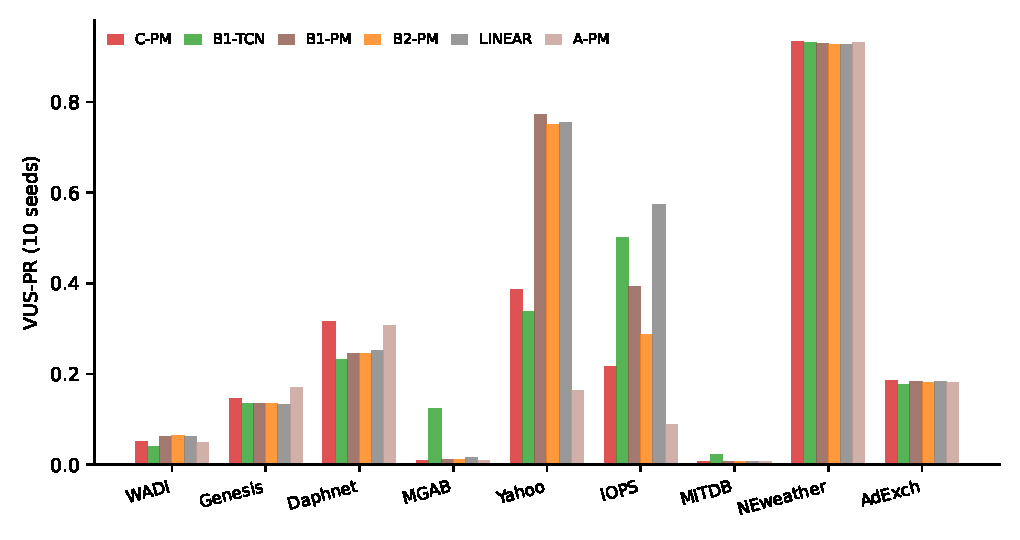
\includegraphics[width=0.9\textwidth]{figures/fig_exclusion_sensitivity.pdf}
\caption{Confirmation stage, per flow: VUS-PR (mean over 10 seeds) for
the five preregistered student arms plus the post-hoc A-PM addition on
the nine held-out sources (the same means as
Table~\ref{tab:confirm}, which additionally appends the teacher and
PCA references). No arm dominates across sources. The best
arm changes from source to source; the macro ordering of the student
arms is unchanged when
the shared-lineage WADI source or the confirmation NAB stream is
excluded.}
\label{fig:confirmflows}
\end{figure}

\subsection{Preregistered Comparisons}\label{sec:confirm-comparisons}
All three preregistered pairwise comparisons are statistically
non-significant at the source level ($n{=}9$; exact two-sided
Wilcoxon signed-rank; the exact test's minimum attainable two-sided
$p$ at $n{=}9$ is 0.0039, which bounds all reported $p$-values from
below). We report raw $p$ first and Holm-adjusted $p$ across the
three-comparison family in brackets. \textbf{B1-TCN vs.\ C-PM}:
mean difference $+0.028$ (bootstrap 95\%~CI $[-0.031,+0.103]$),
$p{=}1.0$ [Holm 1.0], matched-pairs rank-biserial $r{=}-0.02$
(3 wins / 6 losses); the positive mean is driven by a
single source (IOPS, $+0.28$) while C-PM wins pairwise on 6 of 9
sources. \textbf{LINEAR vs.\ C-PM}: $+0.073$
(CI $[-0.014,+0.195]$), $p{=}0.73$ [Holm 1.0], $r{=}+0.16$
(4 wins / 5 losses). \textbf{B2-PM vs.\ B1-PM}: $-0.015$
(CI $[-0.039,+0.000]$), $p{=}0.20$ [Holm 0.60], $r{=}-0.49$
(3 wins / 5 losses / 1 tie): replacing the
self-supervised target by the teacher's forecast provides no detectable
benefit and trends harmful, whereas on the development set the same
macro comparison favored B2-PM by $+0.027$ (0.244 vs.\ 0.217), so the
direction of this (non-significant) contrast is stage-dependent.
A fourth, post-hoc comparison (A-PM vs.\ C-PM: the score vs.\ ranking
interface; exploratory, excluded from the Holm family) is directionally
consistent with the development set
($-0.039$, CI $[-0.097,+0.003]$, $p{=}0.105$, rank-biserial
$-0.62$): the score arm is the weakest of the six student arms in the
confirmation set and the ranking arm the weakest of the five
preregistered ones, completing the score-to-ranking-to-self-supervision
ordering on held-out sources.
Under the preregistered 0.05 VUS-PR margin, the
B2-PM vs.\ B1-PM 95\% CI lies entirely within $\pm0.05$, so
equivalence of the two \emph{training targets} at the mean-source
level is supportable under an interval-based TOST reading (the more
conservative 95\% two-sided CI used here implies the 90\% TOST
criterion is met; $\Delta$ is the mean over the nine sources of the
per-source VUS-PR difference, CIs by source-level bootstrap); the
intervals for
B1-TCN vs.\ C-PM and LINEAR vs.\ C-PM extend to $+0.10$ and $+0.19$
respectively, so the study is underpowered to rule out differences of
that size. Table~\ref{tab:confirmci} consolidates the confirmation-set macro
comparison with flow-level bootstrap intervals, medians, and the three
zero-tuning classical baselines added under revision R11.
The classical additions sharpen the headline.
LOF-window (0.327) and MA-residual (0.325) land above every neural
arm and the fixed PCA baseline, and the frozen teacher itself (0.265)
falls below two zero-tuning methods.
The teacher-distilled arms (C-PM 0.250, A-PM 0.212) close the table's
lower half, so the boundary verdict gains a classical anchor: within
the tested configurations, no teacher signal we can measure survives
transfer as a quality advantage over zero-tuning classical scorers.
As a reference point for statistical power, with $n{=}9$ paired
sources, $\alpha{=}0.05$ two-sided, and 80\% power, the minimum
detectable effect is approximately $0.93\,\sigma_d$ of the paired
differences, about $0.10$ VUS-PR for the observed B1-TCN spread
($\sigma_d{\approx}0.10$) and about $0.15$ for the LINEAR spread
($\sigma_d{\approx}0.16$), matching the upper range the two favorable
CIs allow.

\subsection{Directional Consistency and Practical Reading}\label{sec:confirm-reading}
Although none of the differences is significant on nine sources, the
directional pattern replicates the development set. The two arms that do
not use the teacher's scores, namely LINEAR and B1-PM, have the two highest macro means among the student arms (PCA, a reference, is 0.316)
(macro 0.323 and 0.304 vs.\ 0.250 for the best score-distilled arm), the
forecast-distilled arm sits between (0.289), the score arm A-PM is the
weakest of the six student arms (0.212), and the exploration-stage
champion C-PM is the weakest of the five preregistered arms.
Two sources illustrate the conditional structure. On Yahoo the
self-supervised students dominate everything (B1-PM 0.773 vs.\ teacher
0.301 and C-PM 0.386), whereas on WADI and Genesis the PCA baseline
dominates everything (0.315 and 0.959 vs.\ $\le$0.064 and $\le$0.170
for every other method).
On NEweather every method exceeds 0.92. Exclusion sensitivity. Dropping
the WADI source (iTrust lineage shared with dev SWaT) or the
confirmation NAB stream leaves the arm ordering unchanged (e.g., macro
LINEAR/B1-PM/C-PM = 0.323/0.304/0.250 full, 0.356/0.334/0.275 without
WADI, 0.340/0.319/0.258 without NAB), so neither shared-lineage caveat
drives the directional pattern.
A stratified re-analysis (R10) reinforces this reading.
The confirmation set contains no dead flow on which every method falls
below 0.02 VUS-PR, so the macro comparison is not diluted by
unsignalable sources.
In the four teacher-null flows the strongest teacher-free arms widen
their lead (LINEAR 0.351 versus C-PM 0.165 mean).
In the five sources where the teacher matches or beats the best
self-supervised arm per flow (Genesis, Daphnet, MITDB, NEweather,
NAB-adexchange), score distillation adds only $+0.018$ mean VUS-PR over
that arm, while the fixed PCA baseline still dominates that subgroup
(0.453).
A prospective extension (revision R16) adds one fully independent
tenth source (CATSv2, 153{,}173 test points, 5{,}900 anomalies).
On this source every arm collapses to low absolute levels (0.036 to
0.077), score distillation shows a small edge over self-supervision
(0.077 versus 0.036), and the zero-tuning LOF-window scorer dominates
the source at 0.246.
The primary-set ordering is unchanged on the pooled ten-source sample,
and the boundary verdict gains a classical anchor on new ground.
The neural arms retain one exploratory niche.
On the 66-channel SWaT development source the best self-supervised
student (0.568) exceeds the strongest classical baseline there (PCA at
0.446), an observation we do not extrapolate beyond this source.
Figure~\ref{fig:confirmflows} shows the
per-flow results behind this analysis. The honest summary is twofold:
(i)~\emph{no arm is significantly better than any other at this sample
size}. The study cannot rule out differences of the size the intervals
allow (up to $+0.10$ for B1-TCN vs.\\ C-PM and $+0.19$ for LINEAR
vs.\\ C-PM); and (ii)~across both stages, 29 preregistered flows from 22
original data collections, and 1{,}270 preregistered primary-grid runs
(1{,}856 total including all disclosed controls and additions),
\emph{we find no evidence that a frozen TSFM teacher, through either a
score or a forecast interface, improves a lightweight edge detector
over self-supervised or even linear training under the same budget},
while the fidelity analysis (Section~\ref{sec:dev-fidelity}) shows the
score interface does not even transfer the teacher's ranking behavior.

\subsection{Cost Axis}\label{sec:confirm-cost}

\begin{figure}[t]
\centering
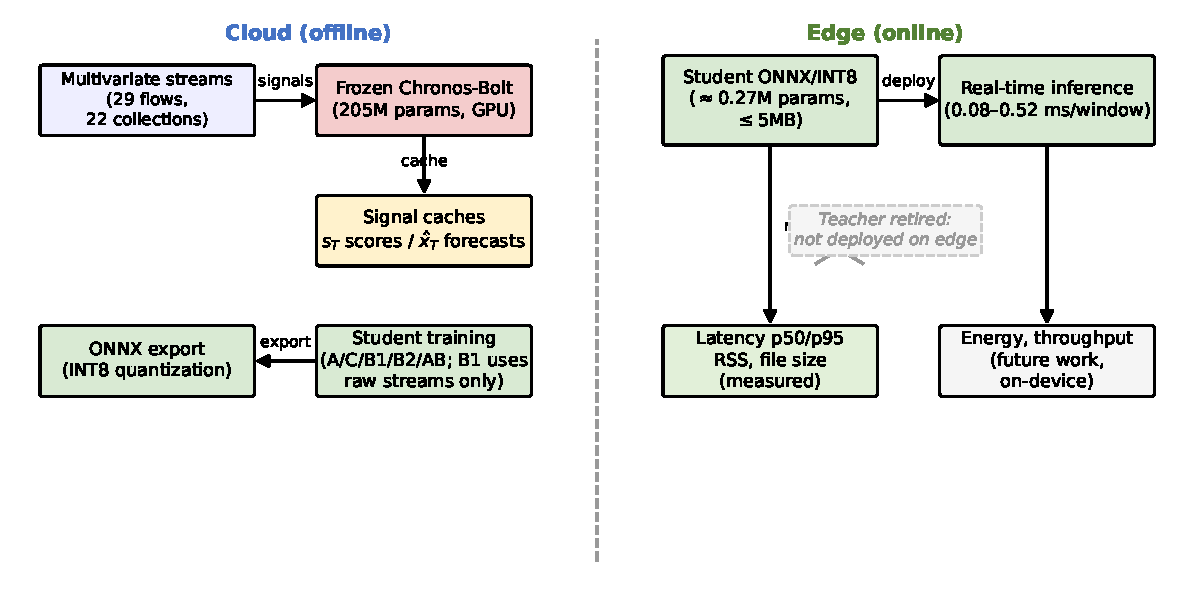
\includegraphics[width=0.95\textwidth]{figures/fig_deployment.pdf}
\caption{Deployment split. All teacher-dependent computation, namely scoring
the training segments and caching its score and forecast
signals, runs offline
in the cloud stage (arm B1 trains on the raw streams alone); the
teacher is retired before deployment. The edge
stage runs the exported student artifact alone ($\approx$0.27M
parameters, ONNX, optional INT8)
and reports the measured quantities of this section (per-window
latency, file size, peak RSS), on the desktop and now also on a
Raspberry~Pi~4B at the reference dimension, including a ten-minute
sustained-throughput check; energy profiling remains future work.}
\label{fig:deployment}
\end{figure}

Two budget tiers anchor the cost axis.
Tier E1 requires a per-window p95 latency below 1\,ms and an
artifact of at most 1\,MB; tier E2 extends both to 5\,ms and
5\,MB.
Thresholds are defined on desktop single-thread measurements; the
Raspberry~Pi~4B figures are device-side validation, not tier
definitions.
The computational budget of the full study is modest.
Building the Chronos-Bolt teacher cache over all thirty flows (twenty-nine
preregistered plus the R16 extension) took 17.4
GPU-hours (mean 35 minutes per flow), a one-time cost shared by every
distilled arm.
Each student training run completes in 1--12 minutes on a single GPU
(mean 84 seconds over the 450 confirmation runs, 12.5 GPU-hours in
total), and the complete 1{,}856-run study fits within roughly 40
GPU-hours of student training plus the cached teacher passes.
All cost figures below are measured on \emph{trained} artifacts
(case-C students retrained once per architecture--dimension
configuration under the confirmation-stage recipe, exported to ONNX,
and re-timed on an idle machine. Appendix~\ref{app:cost} reports the
full matrix with round-to-round ranges). On the desktop CPU
(single-thread ONNX Runtime, batch 1), the
linear floor requires 0.009--0.049\,ms p95 with files at or below
0.13\,MB (budget tier E1 at every dimension). PatchMLP-lite runs in
0.092--0.194\,ms FP32 and, after dynamic INT8 quantization,
0.058--0.116\,ms with 0.22--0.47\,MB files, inside E1 at every tested
dimension (1 to 248 channels). TCN-lite runs in
0.414--0.653\,ms FP32 (E1 at low channel counts by latency; its file
crosses 1\,MB from 66 channels, so E2 there), but its dynamically
quantized variant is 10.3--12.2$\times$ \emph{slower} (quantized
convolution kernels in the runtime), so INT8 is recommended for the
MLP-mixer architecture only. Quantization also perturbs quality. The
INT8-minus-FP32 VUS-PR drift of the exported artifacts is within
$\pm$0.01 on most configurations and even reaches $+0.074$ and $+0.097$
on the 66- and 248-channel PatchMLP students (quantization noise as
regularization), with one loss of $-0.066$ on the 66-channel linear
floor (Appendix~\ref{app:cost}); the linear floor, at most 0.13\,MB,
has no need to quantize.

The frozen teacher (Chronos-Bolt-base) is in a different cost class
entirely. Figure~\ref{fig:deployment} places teacher and student on
opposite sides of the deployment boundary. Its offline scoring pass
over the training segments of all 29 flows cost 15.4 GPU-hours (mean
32 minutes per flow), a one-time cost amortized across every student
trained from the cache, but non-trivial for a single deployment and
zero for self-supervised students. Measured on the same idle machine
(12th-Gen Intel Core
i7-12700F, ONNX Runtime 1.28, PyTorch 2.13; single CPU thread) under
two matching protocols, scoring one point costs 64.7\,ms at batch 64
and 122.9\,ms at batch 1 (the deployment-faithful setting; 512-point
context, end-to-end including normalization and aggregation). The
students' end-to-end cost over full test splits (stride-1 windows,
trained artifacts, two development flows and one held-out
confirmation flow) is 0.07--0.51\,ms p50 per window (p95 up to
0.62\,ms): roughly
\emph{200--1500$\times$} faster than the teacher
at batch 1, depending on architecture and channel count. Combined with
the quality results (Figure~\ref{fig:cost}), the cost axis completes the picture. The teacher is
simultaneously slower than every student by orders of magnitude and not
better than the strongest of them on held-out sources. Peak RSS is
process-level. For the sub-million-parameter students the in-process
delta is below measurement noise ($\le$6\,MB over the ORT runtime
baseline), and cold-start is excluded from the per-window figures (both
disclosed). The Raspberry~Pi~4B on-device measurements follow the identical
protocol (single-thread ONNX Runtime, batch 1, $L=128$, CPU governor
pinned to performance).
On the board, the linear floor measures 0.44\,ms p95, the quantized
PatchMLP student 2.00\,ms, and the TCN student 15.47\,ms at the
66-channel reference.
Process peak RSS stays at 59--62\,MB with no thermal throttling
(49--52$^\circ$C).
These board figures sit 25--33$\times$ above the matching desktop
medians.
The linear floor and the quantized PatchMLP student stay inside their
E1 and E2 budget tiers on the board, while the FP32 TCN student lands
above E2, reinforcing the recommendation to deploy the quantized
MLP-mixer student.
Even on the board, every student remains 8--278$\times$ cheaper than
the teacher's desktop batch-1 cost of 122.9\,ms.
The teacher itself is not deployable on the board at all: Chronos-Bolt-base
requires 2.4\,s per scored point on the same device (batch 1, context
512, end-to-end), roughly 19.5$\times$ its desktop cost and 155 to
5{,}428$\times$ above the student artifacts.


\begin{figure}[t]
\centering
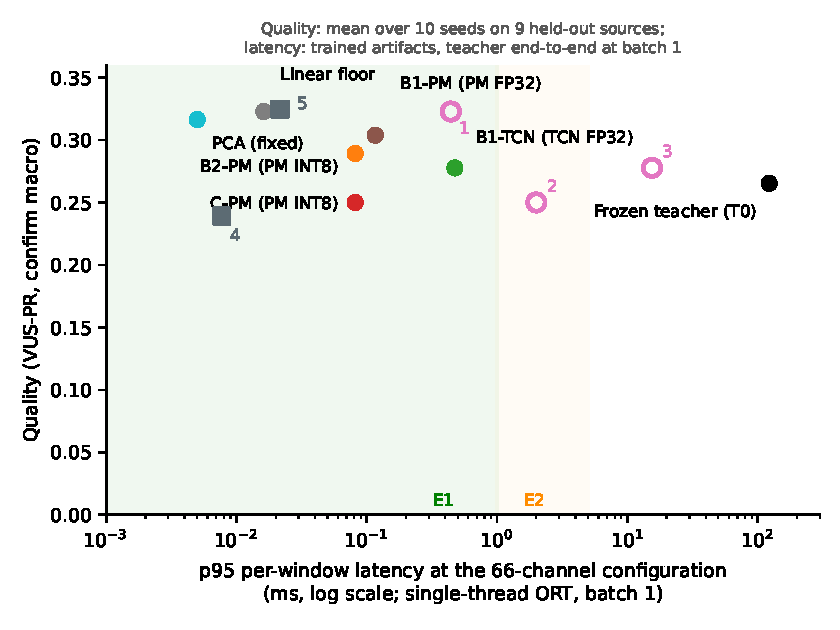
\includegraphics[width=0.85\textwidth]{figures/fig_cost_quality.pdf}
\caption{Cost--quality plane on held-out sources (macro VUS-PR vs.\
single-thread p95 per-window latency at 66 channels, log scale; the
teacher is measured end-to-end at batch 1 (deployment-faithful)). Green and
orange bands are the E1/E2 latency budgets. The teacher sits in a
different cost class entirely; the linear floor and the quantized
PatchMLP students occupy the E1 corner. Pink open squares 1--3 mark the
Raspberry~Pi~4B on-device measurements of the linear floor, quantized
PatchMLP, and TCN students (0.44, 2.00, and 15.47\,ms p95 at the
reference dimension).
Gray squares 4--5 mark the zero-tuning classical scorers Robust-Z
(0.008\,ms) and MA-residual (0.022\,ms p95, streaming,
desktop single-thread).}
\label{fig:cost}
\end{figure}

\section{Discussion}\label{sec:discussion}

\subsection{What Does TSFM Distillation Actually Transfer?}
Our design cannot say what distillation transfers in general, but \emph{here}
it localizes the boundary cleanly. The interface decides. Where fidelity was high, students
cloned the teacher including its weaknesses; where fidelity was near
zero, students diverged from the teacher and typically beat it. Under
the normal-only training constraint, the teacher's scores on clean data
carry little signal that a compact forecaster cannot extract from the
raw series itself. The teacher's failure modes (flat scores,
persistence blind spots) are not worth copying. The forecast target
tells the complementary story: B2 students, trained to predict the
teacher's forecast rather than to mimic its score, close most of the gap
to self-supervision on the development set and show occasional large
wins. In other words, if a
TSFM is in the training loop at all, our development-stage data favor
its \emph{forecasts} over its scores. Detectors trained on either
target are equivalent within the preregistered 0.05 VUS-PR margin on
held-out sources (the interval for the forecast-vs-self-supervision
comparison lies inside the margin), while the score interface is weaker
than both. We emphasize the limitation. Equivalence of the two
\emph{training targets} is what the interval supports, not agreement of
the teacher's forecasts with ground truth. A post-hoc shuffled-teacher
control (revision R6, exploratory; Figure~\ref{fig:shuffle}) sharpens the point. Retraining the
score-distilled student with the teacher's scores randomly permuted
in time (preserving their marginal distribution, destroying their
temporal alignment; A-PM recipe, 2 seeds, all 20 development flows,
bootstrap resampling at the flow level) changes mean VUS-PR by only
$+0.022$ in favor of the true scores (10 wins, 9 losses, 1 tie;
bootstrap 95\% CI of the mean difference $[-0.027, +0.086]$, crossing
zero; exploratory).
The score interface, in this protocol, carries limited information
beyond the marginal distribution of the teacher's scores, though the
interval still allows a mean effect as large as $+0.086$.
Two preregistered controls (R10) probe how general this boundary is.
A capacity sweep over PatchMLP students at 0.27M, 0.6M, 1.6M, and 5.8M
parameters (five development flows, three seeds; the largest size under
revision R13) shows the score-interface deficit narrowing monotonically
with capacity and closing only near six million parameters.
Macro score distillation reaches 0.256 versus 0.346 self-supervised at
0.27M, 0.262 versus 0.342 at 0.6M, 0.291 versus 0.344 at 1.6M, and
0.332 versus 0.343 at 5.8M, where the gap $-0.011$ falls inside the
preregistered 0.05 margin (paired mean difference $-0.011$, bootstrap
95\% CI $[-0.054, +0.030]$, five flows).
The closing size, however, prices itself out of the edge: the exported
5.8M student measures 23.2\,MB FP32 and 5.8\,MB quantized,
4.6 times the E2 storage ceiling in FP32 and just beyond it once quantized,
far outside E1.
Within edge-sized students, the interface, not capacity, is the
binding constraint.
Per-flow ranking fidelity to the teacher spans essentially its whole
range in the same runs (median per-flow $\rho$ from $-0.13$ to $0.99$),
and even at $\rho=0.99$ the distilled student does not exceed
self-supervised training.
Ranking transfer, where it occurs, does not by itself buy quality.

\begin{figure}[t]
\centering
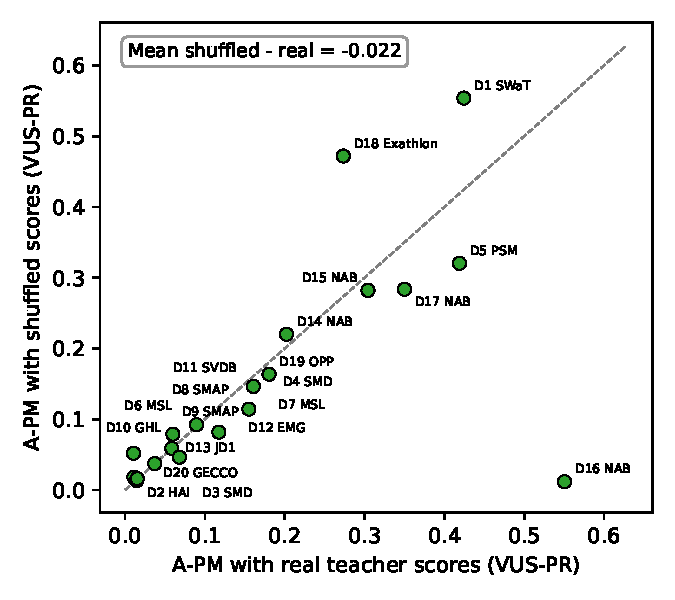
\includegraphics[width=0.7\textwidth]{figures/fig_shuffle_scatter.pdf}
\caption{Shuffled-teacher control (R6, exploratory): per-flow VUS-PR for
A-PM with real teacher scores (x-axis) vs.\ time-shuffled teacher scores
(y-axis; same marginal distribution, destroyed temporal alignment; 2
seeds per flow, paired per flow). The diagonal is $y{=}x$. Real scores
win on 10 flows, lose on 9, tie on 1; mean difference $+0.022$, 95\% CI
$[-0.027, +0.086]$ (flow-level bootstrap), crossing zero.}
\label{fig:shuffle}
\end{figure}
A teacher-on-anomaly control (R8) sharpens this further. Even when the
teacher is given the opportunity to demonstrate anomaly responses in the
training signal, the outcome depends on whether the teacher actually
discriminates those anomalies (Figure~\ref{fig:r8bimodal}). This is
exactly the condition an edge
deployer cannot verify without running the teacher.
A second teacher family (TimesFM 2.5) runs behind the same residual-scoring
structure, with model-specific point forecast extraction (mean output
rather than median quantile) and context length 1024 rather than 512.
The extension was registered over all twenty-nine flows and executed on
thirteen within the compute budget; ten are scorable.
Three streams are shorter than the locked context (1024) and structurally
unscorable for this teacher.
The quality verdict replicates on the ten scorable flows.
The TimesFM-taught student averages 0.239 against 0.372 for the strongest
teacher-free arm, wins one flow in ten, and stays within $\pm 0.03$ of
its Chronos-taught counterpart on seven of ten.
The mechanism picture diverges in one instructive way, read here as an
exploratory case study rather than a controlled strength experiment.
Median ranking fidelity to the TimesFM teacher is 0.70 across 50 runs,
roughly four times the Chronos-side 0.18.
It reaches 0.99 on one development flow where the distilled student
still does not exceed self-supervised training.
Ranking transfer across teacher families is therefore teacher-dependent,
and transfer alone buys no quality.
The TimesFM teacher's own stream-level strength (T0 0.382 vs.\ Chronos
0.069 on SMD) is not converted into student advantage (0.030).
A third family completes the triangle.
Moirai-1.1-R-base (91M, masked-reconstruction architecture, executed under
revision R16 as registered in R9) is distilled through the same score
interface on the same five flows.
Its macro VUS-PR is 0.317, and per-flow ranking fidelity spans -0.20 to
0.83.
The instructive pattern repeats.
On the two flows where fidelity is highest (SVDB $\rho=0.83$, SMD $\rho=0.74$),
quality is lowest (0.058 and 0.036, both below the self-supervised arms).
On the flow where quality is best (SWaT 0.588), fidelity is negative
($\rho=-0.20$).
Three families, three architectures, one conclusion: ranking transfer and
quality gain are decoupled regardless of how much of the teacher's ranking
the student absorbs.
Could a weak teacher explain the boundary instead?
The frozen teacher's confirmation macro (0.265) sits below the linear
floor (0.323), so teacher weakness is a natural confound for the
no-transfer verdict.
Three observations separate the interface account from the
teacher-strength account.
First, within the five sources where the teacher matches or beats the
best self-supervised arm per flow, score distillation still adds only
$+0.018$ mean VUS-PR (group means, exploratory stratification).
Second, the TimesFM extension provides a same-flow natural experiment.
On SMD the two teachers differ fivefold in zero-shot strength (TimesFM
0.382 versus Chronos 0.069), yet their distilled students land within
$0.025$ of each other (0.030 versus 0.055) and both far below the
stronger teacher.
Third, the capacity sweep shows the deficit shrinking smoothly with
student size and closing only near six million parameters, far beyond
the edge budgets at stake.
Teacher strength modulates the ceiling.
Within the tested boundary, the interface is the binding constraint.
These results are included in the artifact package.

\subsection{A Transferability Screening Protocol}
The controls above were run as science, but they double as an engineering
tool.
Before committing a TSFM teacher to a distillation pipeline, a deployer
can screen transferability in three cheap steps, each priced in runs.
Step one is an information probe.
Distill once with time-shuffled teacher scores on a handful of streams
(two seeds, about forty runs in our protocol).
If real and shuffled scores produce indistinguishable students, the
score interface carries nothing beyond the score marginal, and the
teacher earns no place in the loop.
Step two is a capacity probe.
Repeat the score-distilled and self-supervised pair at three student
sizes (about forty-five runs).
A deficit that survives the largest size is an interface property, not a
capacity artifact.
Step three is an interface alternative.
Swap the target to the teacher's forecasts and compare against plain
self-supervision (about thirty runs).
If neither exceeds self-supervision, the teacher can be retired from
training as well as from inference.
The full screen costs about 115 runs, roughly one fifth of the
confirmation budget, and every step reuses cached teacher outputs.
We present it as a screening heuristic derived from this study's controls.
It is not a universal guarantee.

\subsection{Deployment Considerations}
Table~\ref{tab:selection} condenses our results into
hypothesis-generating observations for deployment planning; it is
conditional by design and is \emph{not} a validated decision
procedure. Three practitioner questions frame the table: (i)~Can the
detector be distilled offline, and how large is the artifact that
must reach the device? (ii)~Does the teacher need to accompany the
deployment (it does not, for any student arm)? (iii)~Which anomaly
morphology is expected on the target stream, and does the chosen
arm's failure mode match it? Each table row carries its failure
mode; margins between neural arms are small and not significant.

\begin{table}[t]
\centering
\caption{Practitioner selection table (exploratory; conditional on anomaly morphology and budget; see Section \ref{sec:dev-conditional}).}
\label{tab:selection}
\scriptsize
\begin{tabular}{p{2.7cm}p{3.4cm}p{3.4cm}}
\toprule
Condition & Observed candidate & Failure mode / caveat \\
\midrule
Level or slow-regime anomalies; zero model, zero storage, zero tuning &
MA-residual (causal moving average, $L{=}128$) & Confirmed near the top of the held-out macro (0.325); blind to short micro-transients inside the averaging window \\
Level/regime-shift anomalies; storage $\ge$ a few KB; offline reference OK &
PCA reconstruction (fixed configuration) & Catastrophic on temporal/persistence anomalies (e.g., 0.007 on GHL); reference update needed under drift \\
Tightest latency budget; any morphology except micro-transients &
Linear predictor + residual & Median quality below several neural arms (LINEAR dev macro 0.248 vs.\ B1-TCN 0.253, B2-TCN 0.251); window anomalies near stream start invisible \\
Temporal and persistence anomalies; tightest size budget after INT8 &
B1 (self-supervised) PatchMLP-lite INT8 & Exploratory dev-source niche (SWaT 0.568 vs.\ 0.446 PCA; single-source observation); occupancy edge over C-PM is matched by zero-tuning robust-z \\
Small, smooth-deviation anomalies on short streams (exploratory; not validated on held-out sources) &
Score/ranking-distilled student (C-PM) & Among the weakest arms on held-out sources (macro 0.250; the score arm A-PM is lower at 0.212); margins over B1 are small and not significant; loses the occupancy niche to B1-TCN (B1-TCN 1.000 vs.\ C-PM 0.560 on occupancy) \\
\bottomrule
\end{tabular}
\end{table}

\subsection{Threats to Validity}\label{sec:limitations}
\noindent
We group threats into internal (identification and statistics),
external (generalization), and construct (measurement) validity;
the preregistration revisions R1--R17 and their timing are part of
the internal-validity record.
(1)~The distillation signal exists only on normal-only training segments;
behavioral transfer under real (non-synthetic) anomaly training data remains untested; the synthetic-anomaly control (R8) provides initial evidence.
(2)~Teacher-family checks cover three families.
TimesFM 2.5 (decoder-only) spans ten flows and replicates the no-advantage
verdict with high ranking fidelity (0.70).
Moirai-1.1-R-base (masked-reconstruction, five flows under R16) repeats
the pattern with fidelity up to 0.83.
Three TimesFM streams remain structurally unscorable within the locked
context.
(3)~The preregistration designated causal Matrix Profile and LOF as
auxiliary baselines. Revision R11 added three zero-tuning classical
baselines (robust-z, MA-residual, LOF-window) under the same scoring
protocol; causal Matrix Profile remains unexecuted, as its correct
causal implementation cost remains out of proportion to the question
once three classical controls are present.
(4)~The confirmation set has nine sources. With flow-level bootstrap at
95\%, the observed CI half-widths are 0.05 to 0.10 for neural-arm
contrasts, so the minimum detectable effect is roughly 0.10 to 0.19
VUS-PR on the macro scale. The study rules out differences of that
size and larger, not smaller ones, and all arm-level comparisons are
non-significant at this sample size. Every no-advantage claim in this
paper is bounded by that margin.
(5)~VUS-PR with default buffering is the primary metric; thresholded
operating points and alerting dynamics are out of scope.
(6)~The preregistration was amended five times before any
confirmation-set run (R1--R5) and three more times for exploratory
controls (R6--R8), each disclosed with its trigger and hash
(Appendix~\ref{app:hashchain}); late amendments based on dev-only
evidence are identified as such.
(7)~On-device measurements on a Raspberry~Pi~4B cover latency, memory,
and a ten-minute sustained-throughput check with no thermal throttling
(1800\,MHz throughout, peak 55$\circ$C). Energy profiling remains future
work, and desktop single-thread figures remain the floor for every
other configuration.
(8)~An audit of the training-segment splitter found one development
source (GECCO) whose fallback split places 1.77\% anomalies in its
training segment; excluding it raises every arm's development macro by
0.006 to 0.013 with the ordering unchanged, and the normal-only
descriptions are otherwise accurate (revision R16).

\section{Conclusion}\label{sec:conclusion}
We asked what a frozen TSFM
teacher, what distillation actually transfers, and whether the context
asymmetry drives the outcome.
The answers delineate a boundary rather than a verdict.
First, within the tested boundary, the interface decides what transfers.
The teacher's \emph{score} interface transfers almost none of its
ranking behavior (median $\rho=0.184$, sharply bimodal under anomaly
exposure) and yields no statistically detectable quality benefit.
All preregistered confirmatory tests are non-significant, and the study
rules out large differences only, with CIs extending to $+0.10$ and
$+0.19$ for the two favorable comparisons.
The teacher's \emph{forecast} interface recovers most of the gap on
development flows and is equivalent to self-supervision on held-out
sources, a development-stage preference that did not reach significance
there.
Second, the failure is attributable, not anecdotal.
Shuffled-teacher, equal-context, anomaly-exposure, and
second-teacher-family controls jointly point to the score interface as
the most consistent explanation within the tested teachers, capacities,
and training conditions, without excluding those factors in general.
Third, the deployment case is settled independently of the quality
question.
Students are 200--1500$\times$ cheaper per point than the teacher on
trained artifacts, and quantized PatchMLP students meet
sub-millisecond, sub-megabyte budgets at every tested channel count.
The capacity sweep adds the flip side.
Score distillation closes its deficit to self-supervision only near
six million parameters, whose exported artifact measures 23.2\,MB
(5.8\,MB quantized), so within edge budgets the interface remains
the binding constraint.
The contribution is a disciplined, reproducible boundary delineation
with a mechanism analysis, an interface comparison that redirects
future work toward forecast targets, and a conditional selection
table for practitioners.

\backmatter
\section*{CRediT authorship contribution statement}
\textbf{Yao Zhang:} Conceptualization, Methodology, Software,
Investigation, Data curation, Writing -- original draft, Visualization.
\textbf{Yanling Li:} Supervision, Resources, Writing -- review \& editing.
\textbf{Yichen Wang:} Data curation, Writing -- review \& editing.

\section*{Declaration of generative AI in the writing process}
During the preparation of this work the corresponding author used an AI
assistant (ZCode, GLM) for code development, experiment execution, data
analysis, and drafting support. All experimental decisions followed a
preregistered protocol (v1.0 with append-only revisions R1--R17, released
with the artifacts). The authors verified the results and take full
responsibility for the content of the published article.

\section*{Funding}
The authors received no specific funding for this work.

\section*{Competing interests}
The authors declare no competing interests.

\section*{Data and code availability}
All code (teacher scoring, student training, export/timing, statistics),
the preregistration with its revision log (including the full SHA-256
hash chain of Appendix~\ref{app:hashchain}), per-run results, and the
teacher-score cache metadata are released in the public repository
\url{https://github.com/moonzymoon/tsfm-distillation-artifacts} and
archived with the Zenodo DOI
\url{https://doi.org/10.5281/zenodo.23623799}; the complete
artifact package accompanies the submission. Benchmark data are public (TSB-AD-M, TSB-UAD,
NAB, and the original releases of SMD, PSM, MSL/SMAP, SWaT, HAI 2.2,
MetroPT3, WADI, J-D, EMG, GHL, GECCO, Exathlon, Opportunity, Genesis,
Daphnet, MITDB, SVDB). NAB window labels follow the official combined
label file.

\section*{Acknowledgements}
The teacher-score cache and the detection-interface configuration were
developed within a companion research effort and are reused with
disclosure (Section~\ref{sec:limitations-revision}).

\appendix
\section{Preregistration Revision Log (Hash Chain)}\label{app:hashchain}
\begin{table}[t]
\centering
\scriptsize
\caption{Preregistration revision log (hash chain). Each row records one
append-only revision of the preregistration document; the hash column gives
the first 16 hex characters of the SHA-256 digest of the registered file.}
\label{tab:hashchain}
\begin{tabular}{lllp{4.2cm}}
\toprule
Rev. & Date/Time & SHA-256 (first 16 hex) & Trigger \\
\midrule
v1.0 & 2026-10-03 00:23 & 315881ad7321641f & initial freeze, before any test metric \\
R1 & 2026-10-03 01:40 & 7e6f55158c350fb9 & smoke-test metadata corrections \\
R2 & 2026-10-03 12:13 & 14f2dea01a2fcf07 & WADI format, NAB label, ordering fixes \\
R3 & 2026-10-04 09:17 & ed9ab91e219d26f2 & AB-arm deviation; two-arm confirmation amendment \\
R4 & 2026-10-04 21:02 & 1948c19c4ff8ff2d & C9 replacement, CPU execution mode \\
R5 & 2026-10-04 22:50 & 6afbb2cc0720e685 & five-arm confirmation amendment; MP/LOF non-execution disclosure \\
R6 & 2026-10-06 09:36 & 69177d7d3ae715b8 & shuffled-teacher exploratory control (recorded post-hoc) \\
R7 & 2026-10-06 21:17 & d9bacd89964b7c65 & interface ablation at teacher context length (recorded pre-run) \\
R8 & 2026-10-07 22:37 & ab88763bbd684611 & teacher-on-anomaly distillation control (recorded pre-run) \\
R9 & 2026-10-08 23:33 & d7f5d4e347cbc308 & Moirai third-teacher control (registered pre-run; not executed) \\
R10 & 2026-10-13 01:08 & 9a8a606d3a3686e5 & submission-hardening controls: second-teacher full-flow, capacity sweep, stratified macro \\
R11 & 2026-10-17 09:21 & 74143d38e48c8184 & classical baselines (robust-z, MA-residual, LOF-window) and presentation hardening \\
R12 & 2026-10-17 09:37 & f7d87930c89216b5 & erratum: R11 timing-evidence wording corrected \\
R13 & 2026-10-17 10:04 & 8284d2bac26f3625 & capacity sweep extension to 5.8M parameters (pre-run) \\
R14 & 2026-10-17 22:58 & 0f3fd5a2b282210a & classical-baseline latency measurement and cost-plane update (pre-run) \\
R15 & 2026-10-18 01:42 & 30ba2d792c9cff3f & on-device sustained-throughput and teacher-latency measurements (pre-run) \\
R16 & 2026-10-18 23:40 & af2f5824507d6682 & leakage audit disclosure, Moirai third-family execution, prospective tenth-source extension, stratified re-analysis \\
R17 & 2026-10-19 00:22 & f61d9c351fb91c1f & R16 candidate-source erratum: CreditCard, CATSv2, TAO, LTDB \\
\bottomrule
\end{tabular}
\end{table}
Each revision is append-only; the confirmation data were untouched until
after R5. Table~\ref{tab:hashchain} lists all eighteen revisions
with their registered hashes. Revisions R1--R5 were registered before any confirmation-set
run. R6--R8 are exploratory controls registered post-hoc (R6) or
pre-run for post-hoc experiments (R7, R8), as flagged in the trigger
column.
R9 registered a third-teacher (Moirai) control that stayed unexecuted
until R16 carried it out on five flows.
R10 registers the submission-hardening controls, covering a
capacity-interface sweep registered before its runs, a second-teacher
full-flow extension registered mid-execution before any result was
inspected, and a post-hoc stratified re-analysis.
The preregistration text, this hash chain, and all per-run
results are part of the artifact package.
The chain evidences disclosure transparency.
Full-length hashes and file timestamps are in the artifact package, and
no external timestamping authority is claimed.

\section{Reproduction Details}\label{app:repro}
Table~\ref{tab:repro} summarizes the reproduction configuration.
\begin{table}[t]
\centering
\scriptsize
\caption{Reproduction details.}\label{tab:repro}
\begin{tabular}{p{3.7cm}p{3.5cm}p{3.5cm}}
\toprule
Item & Value & Source \\
\midrule
Student backbones & TCN-lite: 4-stage dilated causal conv (96/112/128/128, kernel 5), pool-4 head; PatchMLP-lite: patch 8 (PatchTST~\cite{nie2023patchtst}), dim 128, 2 mixer blocks (MLP-Mixer~\cite{tolstikhin2021mixer}) & artifact code \\
Parameters (66-ch instance) & TCN-lite 272{,}401; PatchMLP-lite 265{,}617; linear floor 8{,}383 & counted at build \\
Training & Adam, lr $10^{-3}$, batch 256, 30 epochs, window $L{=}128$, stride 2, per-flow & run manifests \\
Teacher scoring & context 512 (Chronos-Bolt) / 1024 (TimesFM 2.5); point forecast = median quantile (Chronos) or mean output (TimesFM) & cache metadata \\
Export & ONNX opset 17; dynamic batch; optional dynamic INT8 & timing script \\
Run ledger & 1{,}856 total: 1{,}270 preregistered (400 main grid + 420 auxiliary + 450 five-arm confirmation) + 586 post-hoc/controls and additions (90 A-PM confirmation addition + 40 shuffled-teacher R6 + 25 TimesFM subset + 30 interface ablation R7 + 30 anomaly-exposure R8 + 25 TimesFM full-flow R10 + 135 capacity-sweep R10 + 87 classical-baseline scoring R11 + 45 capacity-1024 R13 + 60 extension-arm R16 + 4 extension-evaluation R16 + 15 Moirai R16). Fig.~3 plots all runs with finite fidelity: 389 main-grid plus 420 auxiliary runs & per-run manifests \\
\bottomrule
\end{tabular}
\end{table}

\section{Deployment-Cost Matrix on Trained Artifacts}\label{app:cost}
Table~\ref{tab:costmatrix} reports the full per-configuration cost
matrix: three architectures at six channel counts (1, 9, 38, 66, 116,
248, each realized on a real flow of that dimensionality), FP32 and
dynamic-INT8 variants, five timing rounds each. The timing artifacts
are case-C students retrained under the confirmation recipe for this
matrix; latency depends on the computation graph (architecture,
dimension, precision), not on weight values, and the quality-drift
column verifies that the deployed artifacts retain detection behavior.
The end-to-end protocol (stride-1 windows over full test splits,
single-thread, batch 1) was additionally measured on two development
flows (NAB cpu, SMD) and one held-out confirmation flow (Daphnet):
PatchMLP 0.069--0.084\,ms p50, TCN 0.329--0.511\,ms p50.

% AUTO-GENERATED from results/cost/timing_matrix_TRAINED.json — do not edit
\begin{table}[t]
\centering
\caption{Deployment-cost matrix on trained artifacts (case-C students, seed 0, M6 training protocol; idle desktop CPU, single-thread ONNX Runtime, batch 1, window $L{=}128$; median over 5 rounds of 50 warm-up + 500 timed windows, with round-to-round min--max of p95 in parentheses. The final column gives the INT8-minus-FP32 VUS-PR drift of the exported artifacts on each flow's test split.}
\label{tab:costmatrix}
\scriptsize
\setlength{\tabcolsep}{3.5pt}
\begin{tabular}{llrrrrrr}
\toprule
Ch & Model & Prec & p50 (ms) & p95 (ms) & p95 range & MB & $\Delta$VUS \\
\midrule
1 & LINEAR & FP32 & 0.009 & 0.009 & 0.009--0.013 & 0.00 & ref \\
1 & LINEAR & INT8 & 0.010 & 0.010 & 0.010--0.011 & 0.00 & +0.000 \\
\addlinespace[2pt]
1 & PatchMLP & FP32 & 0.073 & 0.092 & 0.072--0.169 & 0.80 & ref \\
1 & PatchMLP & INT8 & 0.055 & 0.058 & 0.056--0.064 & 0.22 & +0.000 \\
\addlinespace[2pt]
1 & TCN & FP32 & 0.346 & 0.452 & 0.437--0.473 & 0.97 & ref \\
1 & TCN & INT8 & 4.315 & 4.653 & 4.550--4.778 & 0.26 & -0.000 \\
\addlinespace[2pt]
9 & LINEAR & FP32 & 0.009 & 0.010 & 0.009--0.011 & 0.01 & ref \\
9 & LINEAR & INT8 & 0.011 & 0.011 & 0.011--0.011 & 0.00 & -0.002 \\
\addlinespace[2pt]
9 & PatchMLP & FP32 & 0.077 & 0.092 & 0.079--0.168 & 0.83 & ref \\
9 & PatchMLP & INT8 & 0.060 & 0.072 & 0.061--0.093 & 0.22 & +0.005 \\
\addlinespace[2pt]
9 & TCN & FP32 & 0.335 & 0.414 & 0.386--0.432 & 0.98 & ref \\
9 & TCN & INT8 & 4.109 & 4.391 & 4.341--4.512 & 0.26 & -0.009 \\
\addlinespace[2pt]
38 & LINEAR & FP32 & 0.012 & 0.013 & 0.013--0.019 & 0.02 & ref \\
38 & LINEAR & INT8 & 0.013 & 0.014 & 0.014--0.014 & 0.01 & +0.000 \\
\addlinespace[2pt]
38 & PatchMLP & FP32 & 0.091 & 0.108 & 0.102--0.121 & 0.95 & ref \\
38 & PatchMLP & INT8 & 0.066 & 0.072 & 0.069--0.082 & 0.25 & -0.000 \\
\addlinespace[2pt]
38 & TCN & FP32 & 0.363 & 0.429 & 0.416--0.444 & 1.04 & ref \\
38 & TCN & INT8 & 4.544 & 4.842 & 4.821--4.916 & 0.28 & -0.001 \\
\addlinespace[2pt]
66 & LINEAR & FP32 & 0.016 & 0.016 & 0.016--0.020 & 0.03 & ref \\
66 & LINEAR & INT8 & 0.016 & 0.016 & 0.016--0.016 & 0.01 & -0.066 \\
\addlinespace[2pt]
66 & PatchMLP & FP32 & 0.099 & 0.116 & 0.106--0.120 & 1.07 & ref \\
66 & PatchMLP & INT8 & 0.069 & 0.082 & 0.077--0.094 & 0.28 & +0.074 \\
\addlinespace[2pt]
66 & TCN & FP32 & 0.388 & 0.474 & 0.450--0.508 & 1.09 & ref \\
66 & TCN & INT8 & 4.943 & 5.460 & 5.379--5.567 & 0.29 & +0.048 \\
\addlinespace[2pt]
116 & LINEAR & FP32 & 0.023 & 0.024 & 0.024--0.025 & 0.06 & ref \\
116 & LINEAR & INT8 & 0.020 & 0.023 & 0.022--0.024 & 0.02 & +0.000 \\
\addlinespace[2pt]
116 & PatchMLP & FP32 & 0.113 & 0.142 & 0.130--0.147 & 1.27 & ref \\
116 & PatchMLP & INT8 & 0.078 & 0.085 & 0.080--0.093 & 0.33 & +0.000 \\
\addlinespace[2pt]
116 & TCN & FP32 & 0.438 & 0.531 & 0.521--0.537 & 1.19 & ref \\
116 & TCN & INT8 & 5.710 & 6.052 & 6.020--6.159 & 0.31 & -0.002 \\
\addlinespace[2pt]
248 & LINEAR & FP32 & 0.047 & 0.049 & 0.046--0.057 & 0.13 & ref \\
248 & LINEAR & INT8 & 0.033 & 0.035 & 0.033--0.037 & 0.03 & +0.009 \\
\addlinespace[2pt]
248 & PatchMLP & FP32 & 0.158 & 0.194 & 0.176--0.199 & 1.81 & ref \\
248 & PatchMLP & INT8 & 0.105 & 0.116 & 0.113--0.136 & 0.47 & +0.097 \\
\addlinespace[2pt]
248 & TCN & FP32 & 0.561 & 0.653 & 0.634--0.769 & 1.44 & ref \\
248 & TCN & INT8 & 7.640 & 7.995 & 7.989--8.034 & 0.38 & +0.002 \\
\addlinespace[2pt]
\bottomrule
\end{tabular}
\end{table}

% bibstyle set via class option sn-basic
\bibliography{refs}

\end{document}
